\documentclass[APA,STIX1COL]{WileyNJD-v2}
\usepackage[utf8]{inputenc}
\usepackage{siunitx}
\sisetup{group-digits=false}
\renewcommand{\thefigure}{\arabic{figure}}
\renewcommand{\thetable}{\arabic{table}}
\usepackage{graphicx}
\usepackage{subcaption}
\usepackage{array}
\captionsetup[figure]{labelsep=quad}
\captionsetup[table]{labelsep=quad}
\usepackage[section]{placeins}
\usepackage{float}        % for [H] placement
\usepackage{threeparttable}

\usepackage{soul}

% Figures/ is the manuscript's canonical asset tree.
\graphicspath{
  {Figures/manuscript/}
  {Figures/appendix_cutoff_panels/}
  {Figures/multivariate_synthesis_by_cutoff/}
}

\articletype{Research Article} % Specify article type

\historydates{}
\doiheadtext{}
\copyyear{2025}
\startpage{1}

\raggedbottom
\hypersetup{hidelinks}
% The unpublished draft has no journal volume, page range, or citation box.
\renewcommand{\printjnlcitation}{}

%%%%%%%%%%%%%%%%%%%%%%%%%%%%%%
% My commands:
\newcommand*\mymin[1][]{\min_{#1}\,}
\newcommand{\vect}[1]{\mathbf{#1}}
\newcommand\numberthis{\addtocounter{equation}{1}\tag{\theequation}}
\newcommand\independent{\protect\mathpalette{\protect\independenT}{\perp}}
\def\independenT#1#2{\mathrel{\rlap{$#1#2$}\mkern2mu{#1#2}}}

\newcommand{\bs}[1]{{\textcolor{blue}{#1}}}
%%%%%%%%%%%%%%%%%%%%%%%%%%%%%%

\begin{document}

\title{Bayesian Quantile-Based Correction and Synthesis of Hydrologic Products}

\author[1]{Antonio De Leon*}
\author[1]{Raquel Prado}
\author[1]{Bruno Sans\'o}

\authormark{De Leon \textsc{et al.}} % Running head author name

\address[1]{\orgdiv{Department of Statistics}, \orgname{University of California, Santa Cruz}, \orgaddress{\state{California}, \country{USA}}}

\corres{*Corresponding author: Antonio De Leon. \email{jaguir26@ucsc.edu}}

\presentaddress{University of California, Santa Cruz, Santa Cruz, CA, USA.}

\abstract[Summary]{We develop a Bayesian correction-and-synthesis framework using dynamic quantile linear models for river-flow forecasting. A shared latent quantile process relates gauge observations, retrospective products and forecast ensembles through source-specific dynamic discrepancies, accommodating different product horizons. Our predictive synthesis combines full predictive distributions from separate quantile fits into a nondecreasing marginal quantile function, including tails beyond the fitted probabilities. We develop Laplace--Delta variational Bayes (VB) computation with joint non-conjugate scale and skewness updates for the extended dynamic quantile linear model. We illustrate the method with daily San Lorenzo River flow, combining U.S. Geological Survey observations with European Centre for Medium-Range Weather Forecasts Global Flood Awareness System products and National Oceanic and Atmospheric Administration National Weather Service products. Across five forecast origins, the reference specification reduces mean continuous ranked probability score relative to seasonal climatology by 68.6\% over 28 days and 59.0\% over eight days on the log-transformed discharge scale. Its central 95\% predictive intervals cover 87.9\% and 72.5\% of cases, respectively.}

\keywords{Bayesian forecasting, quantile regression, dynamic models, river flow prediction}

\maketitle


\section{INTRODUCTION}
\label{sec:introduction}

River-flow forecasts support flood preparedness, drought monitoring, reservoir operations and water-supply planning. These decisions require predictive distributions that describe routine conditions and extremes. Hydrological uncertainty arises from imperfect observations, model structure, parameters and initial states. Meteorological uncertainty enters through precipitation and other atmospheric forcing as weather inputs propagate through a catchment \citep{thiboult2016accounting,tarek2021daily}. Operational forecasts use conceptual and physically based hydrological models whose calibration and implementation shape this propagation \citep{demargne2013science}. Statistical correction must relate their output to the flow observed at a gauge while representing predictive uncertainty.

Forecast combination and statistical post-processing offer established approaches \citep{siegert2019forecast,vannitsem,wang2022forecastcombinations50yearreview}. Bayesian model averaging combines hydrological predictive distributions \citep{duan2006bma}; ensemble model output statistics (EMOS) relates distribution parameters to ensemble forecasts \citep{gneiting2005emos}, including location and spread corrections in hydrology \citep{hemri2015multivariate}. Quantile methods have been used to merge precipitation products \citep{yumnam2022quantile}, and dynamic Bayesian predictive synthesis combines information over time \citep{mcalinn2019dynamic}. The products available here differ in spatial support, horizon and update frequency. A joint model should distinguish observations, retrospective products and issued ensembles while allowing their discrepancies from the target river-flow process to evolve.

Within dynamic quantile linear models (DQLMs; \citealp{gourieroux2008dqlm,goncalves,barata2021_flex_quantile}), we make three contributions. First, a shared latent quantile process relates gauge measurements to products with different horizons through source-specific dynamic discrepancies. Second, synthesis combines full predictive distributions from separate quantile fits, including their tails, into a nondecreasing marginal quantile function. Third, we adapt Laplace--Delta approximations \citep{wang2013nonconjugatevb} for joint non-conjugate scale and skewness updates within variational Bayes (VB) filtering and smoothing for the extended DQLM. This makes multi-decade daily analyses practical. Correction combines sources within fits; synthesis combines their predictive distributions.

The application concerns San Lorenzo River flow at Big Trees, California. We combine U.S. Geological Survey (USGS) observations with European Centre for Medium-Range Weather Forecasts (ECMWF) Global Flood Awareness System (GloFAS) products and National Oceanic and Atmospheric Administration (NOAA) National Weather Service (NWS) products. Five origins provide 28-day and common eight-day comparisons using the continuous ranked probability score (CRPS), targeted quantile losses and predictive calibration. Sections~\ref{sec:data}--\ref{sec:evaluation} describe the data, method and evaluation; Section~\ref{sec:forecastvalidation} reports the findings and Section~\ref{sec5} discusses their implications. Appendices~\ref{app:datahistories}--\ref{app:vbupdates} provide data-source details, additional results and computational specifications.

\section{FORECASTING SETTING AND DATA}
\label{sec:data}

\subsection{Study Setting and Observations}

The target is daily mean San Lorenzo River discharge at the USGS Big Trees gauge, station 11160500, Santa Cruz, California (Figure~\ref{fig:sanlorenzo}; \citealp{usgs_daily_11160500}). The record contains 12,995 daily observations from May 29, 1987 through December 25, 2022. We convert cubic feet per second to m$^3$/s and model $\log(1+x)$, where $x$ is discharge in m$^3$/s. The record spans prolonged dry conditions and winter high-flow episodes.

\begin{figure}[!htbp]
\centering
\includegraphics[width=450pt]{site_context_usgs.png}
\caption{USGS daily discharge, May 29, 1987 through December 25, 2022, on the $\log(1+x)$ scale with $x$ in m$^3$/s. Dashed lines are approximate current-rating discharge equivalents of current NWS minor and major stage categories at BTEC1/USGS 11160500, computed from USGS rating 40.0 \citep{cnrfc_btec1,usgs_11160500_rating40}. They give magnitude references rather than historical flood-stage classifications of daily means.}
\label{fig:sanlorenzo}
\end{figure}

A forecast origin, or cutoff, is denoted by $T$; the first target is $T+1$. Paired gauge and retrospective records estimate each source's discrepancy before $T$. External ensembles then inform future flow through the discrepancy-adjusted channels. Precipitation, soil moisture and a climate summary enter a separate transfer component of the latent quantile process.

\subsection{External Products and Covariates}

The base transfer inputs are local precipitation from the Parameter-elevation Regressions on Independent Slopes Model (PRISM) Climate Group \citep{prism}, soil moisture from ECMWF ERA5-Land \citep{ecmwf,munozsabater2021era5land}, and broader climate information. Historical precipitation and soil moisture are extracted at the gauge location; forecast-window paths include Global Ensemble Forecast System (GEFS) precipitation and shallow soil-water forecasts. Precipitation enters as a covariate, including on dry days, without a separate occurrence model. ERA5-Land supplies a reanalysis-based land-state covariate with uncertainty; USGS discharge supplies the verification target.

Monthly NOAA Physical Sciences Laboratory climate-index series \citep{noaa_climate_indices} are interpolated to daily resolution and standardized. Their first generalized dynamic principal component (GDPC; \citealp{JSSv092c02}) explains 44.07\% of total index variability and provides the climate covariate. Appendix~\ref{app:datahistories} lists the indices, spatial extraction and product versions, and displays the historical inputs.

GloFAS \citep{harrigan2020glofas} and NWS, including NOAA National Water Model (NWM) output \citep{cosgrove2024noaa}, each contribute retrospective discharge and an issued ensemble. GloFAS has 51 members over 28 days. The NWS ensemble has seven members: six extend to 8.5 days and one control to ten days; the daily analysis retains eight valid leads. At the representative December 25, 2022 origin, these horizons end on January 22 and January 2, 2023, respectively. Source availability determines which observation channels enter at each lead. Source versions and extraction records accompany the analysis data \citep{deleon2026sanlorenzo_reproducibility}.
\section{BAYESIAN CORRECTION AND PREDICTIVE SYNTHESIS}
\label{sec:methodology}

For each target probability $p_0$, dynamic correction combines the source channels within a quantile fit; synthesis combines predictive distributions across fits. We distinguish the conditional model quantile given states and likelihood parameters, a posterior predictive quantile integrating their uncertainty, and the synthesized predictive quantile. Bold symbols denote vectors or matrices; $\mathbf I_r$, $\mathbf 0_r$ and $\mathbf 1_r$ denote the $r$-dimensional identity, zero vector and one vector.

\subsection{Quantile Likelihood}
\label{subsec:exal}

The asymmetric Laplace (AL) distribution provides a working likelihood for Bayesian quantile inference \citep{yu2001bayesian, sriram2013theoretical}. We use the extended asymmetric Laplace (exAL) distribution, \(\operatorname{exAL}_{p_0}(\mu,\sigma,\gamma)\), developed by \citet{yan2025new}. Its location \(\mu\) is the \(p_0\)-quantile, \(\sigma>0\) controls scale, and \(\gamma\) provides additional skewness flexibility. To preserve the specified quantile, \(\gamma\) lies in an interval \((L_\gamma(p_0),U_\gamma(p_0))\) whose endpoints depend on \(p_0\). Subsection~\ref{app:augmentation} gives the endpoints and computational augmentation.

\subsection{State-Space Model Specification}
\label{subsec:fullmodel}

The transformed-discharge process spans the observation period and forecast horizon. The shared trend and seasonal state is $\boldsymbol\theta_t\in\mathbb R^p$, with loading $\mathbf F_t\in\mathbb R^p$. Each source $j\in\mathcal J=\{1,\ldots,J\}$ has a discrepancy state $\boldsymbol\delta_t^j\in\mathbb R^p$. A scalar transfer state $\zeta_t$ incorporates covariates $\mathbf x_t\in\mathbb R^m$ with time-varying coefficients $\boldsymbol\psi_t\in\mathbb R^m$. Source $j$ has members $i\in\mathcal I_j=\{1,\ldots,I_j\}$ and leads $k\in\mathcal K_j=\{1,\ldots,K_{(j)}\}$; let $K_{\max}=\max_jK_{(j)}$.

Write $y_t^o$ for gauge observations, $z_t^j$ for retrospective source discharge and $y_T^{j,i}(k)$ for member $i$'s forecast issued at $T$ for lead $k$, all on the $\log(1+x)$ scale. Conditional on states and channel parameters, the observation channels are independent:
\begin{alignat}{3}
\text{Observed measurements:}\quad&
y_t^o
&\sim{}& \text{exAL}_{p_0}\!\left(\mathbf{F}_t' \boldsymbol{\theta}_t + \zeta_t, \sigma^0, \gamma^0\right),
&\qquad& 1 \le t \le T, \label{eq:unified_usgs}
\\
\text{Retrospective products:}\quad&
z_t^j
&\sim{}& \text{exAL}_{p_0}\!\left(\mathbf{F}_t'(\boldsymbol{\theta}_t + \boldsymbol{\delta}_t^j) + \zeta_t, \sigma^j, \gamma^j\right),
&\qquad& j \in \mathcal{J},\ 1 \le t \le T, \label{eq:unified_retro}
\\
\text{Forecast products:}\quad&
y_T^{j,i}(k)
&\sim{}& \text{exAL}_{p_0}\!\left(\mathbf{F}_{T+k}'(\boldsymbol{\theta}_{T+k} + \boldsymbol{\delta}_{T+k}^j) + \zeta_{T+k}, \sigma^j, \gamma^j\right),
&\qquad& j \in \mathcal{J},\ i \in \mathcal{I}_j,\ k \in \mathcal{K}_j, \notag
\\
\text{Trend and seasonal states:}\quad&
\boldsymbol{\theta}_t \mid \boldsymbol{\theta}_{t-1}
&\sim{}& \mathcal{N}\!\left(\mathbf{G}_t \boldsymbol{\theta}_{t-1}, \mathbf{W}_t^\theta\right),
&\qquad& 1 \le t \le T+K_{\max}, \label{eq:unified_theta}
\\
\text{Discrepancy states:}\quad&
\boldsymbol{\delta}_t^j \mid \boldsymbol{\delta}_{t-1}^j
&\sim{}& \mathcal{N}\!\left(\mathbf{G}_t \boldsymbol{\delta}_{t-1}^j, \mathbf{W}_t^{\delta^j}\right),
&\qquad& j \in \mathcal{J},\ 1 \le t \le T+K_{\max}, \label{eq:unified_delta}
\\
\text{Transfer adjustment:}\quad&
\zeta_t \mid \zeta_{t-1}, \boldsymbol{\psi}_{t-1}
&\sim{}& \mathcal{N}\!\left(\lambda \zeta_{t-1} + \mathbf{x}_t'\boldsymbol{\psi}_{t-1}, w_t^\zeta\right),
&\qquad& 1 \le t \le T+K_{\max}, \label{eq:unified_transfer}
\\
\text{Covariate-effect states:}\quad&
\boldsymbol{\psi}_t \mid \boldsymbol{\psi}_{t-1}
&\sim{}& \mathcal{N}\!\left(\boldsymbol{\psi}_{t-1}, \mathbf{W}_t^\psi\right),
&\qquad& 1 \le t \le T+K_{\max}. \notag
\end{alignat}

The conditional gauge quantile is $\mu^o_{p_0,t}=\mathbf F_t'\boldsymbol\theta_t+\zeta_t$; source quantiles additionally contain $\mathbf F_t'\boldsymbol\delta_t^j$. The transition $\mathbf G_t$ and covariances $\mathbf W_t^\theta,\mathbf W_t^{\delta^j}$ are $p\times p$, $\mathbf W_t^\psi$ is $m\times m$, and $w_t^\zeta>0$ is scalar. The persistence parameter $\lambda\in\mathbb R$ and $\mathbf x_t'\boldsymbol\psi_{t-1}$ govern the transfer update; $\mathbf x_{T+k}$ is the supplied lead-$k$ vector.

Historical channels comprise the gauge and retrospective products; future channels comprise available forecast members. Shared states induce dependence after integration, although the working likelihood assumes conditionally independent member residuals. Member counts, source scales and augmentation precisions jointly determine information contributions, rather than a fixed source-weight ratio. Retrospective and forecast products share source-specific scale and skewness without a lead index. Predictive uncertainty can nevertheless change through the states, covariances and source availability. Residual member correlation and lead-dependent observation scales are not explicitly modeled.

For prior specification and computation, stack the components as
\[
\boldsymbol\eta_t'=[\boldsymbol\theta_t',\ (\boldsymbol\delta_t^1)',\ldots,(\boldsymbol\delta_t^J)',\ \zeta_t,\ \boldsymbol\psi_t'],
\qquad q=(J+1)\cdot p+m+1.
\]
Let $\mathcal J_0=\{0\}\cup\mathcal J$, with channel 0 denoting the gauge. Subsection~\ref{app:stackedstates} gives the selectors and block matrices; the component equations above identify the modeling roles assessed in Subsection~\ref{subsec:comparisonspecifications}.

\subsection{Prior Specification and Discounting}
\label{subsec:prioranddisc}
Following \citet{barata2021_flex_quantile}, assign channel-specific truncated Student-$t$ skewness priors and inverse-gamma scale priors,
\[
\gamma^s\sim t_{(L_\gamma(p_0),U_\gamma(p_0))}(0,\phi^s,\nu^s),\qquad
\sigma^s\sim IG(a_{\sigma^s},b_{\sigma^s}),\qquad s\in\mathcal J_0,
\]
where $\phi^s,\nu^s$ are scale and degrees of freedom and $a_{\sigma^s},b_{\sigma^s}$ are shape and scale. Initialize the full state as $\boldsymbol\eta_0\sim\mathcal N(\mathbf m_0,\mathbf C_0)$, with $q$-dimensional mean and $q\times q$ covariance.

Component discount factors \citep{prado2021time} control evolution variances: values lie in $(0,1]$, with 1 suppressing evolution and smaller values allowing adaptation. In forecasting, an inverse-Wishart prior stabilizes evolution covariance around $c\mathbf W_T$, where $c>0$ rescales the origin covariance. The origin covariance is carried forward as a reference: the posterior mean gives it weight $\epsilon/(1+\epsilon)$ and the expected state-innovation covariance weight $1/(1+\epsilon)$, for $\epsilon>0$. Subsection~\ref{app:forecastcovariance} gives the full specification and active-state dimensions; Subsection~\ref{subsec:specification} gives application settings.

\subsection{Posterior Computation}
\label{subsec:postinf}

The AL and exAL fits use mean-field VB; Gaussian variants use Gaussian filtering and smoothing. The approximation separates the joint Gaussian state trajectory, observation-specific augmentation factors and channel-specific scale--skewness factors. Conditional Gaussian augmentation permits variational filtering and smoothing. Coordinate ascent alternates state updates using expected precisions and precision-weighted offsets, generalized inverse-Gaussian and positive-truncated normal augmentation updates, and joint scale--skewness updates. For the latter, VB Laplace--Delta (VB-LD) matches a mode and curvature on an unconstrained parameterization; a second-order Delta approximation supplies nonlinear expectations \citep{wang2013nonconjugatevb}. Changes in the evidence lower bound (ELBO), states, scales and skewness determine stopping after required minimum update counts. Subsection~\ref{app:vblad} and Appendix~\ref{app:vbupdates} give the factorization, formulas and update sequence, including forecast-member contributions.

This extends \citet{barata2021_flex_quantile}, whose importance-sampling treatment fixes scale using an AL fit, by approximating scale and skewness jointly. The intended daily forecast cycle requires posterior updates to finish within a day. For the full record of 12,995 daily observations, a 34-dimensional state and seven quantile models, we expect a full-data Markov chain Monte Carlo (MCMC) analysis to require several weeks of computation because of repeated sampling of latent trajectories, observation-specific augmentation variables and non-conjugate parameters. This is a runtime estimate, rather than a measured MCMC timing. Parallel VB computation with the R package \texttt{exdqlm} \citep{deleon2026exdqlm} gives a representative combined fitting and forecasting time of approximately two hours under the conditions in Subsection~\ref{app:computationtime}. A corresponding full-model MCMC comparison has not been performed, so variational posterior approximation error remains unquantified by the predictive assessments.

\subsection{Posterior Predictive Synthesis Across Quantiles}
\label{subsec:quantilesynthesis}

The quantile-specific model with source-specific discrepancies is fitted separately at probabilities \(0<\tau_1<\cdots<\tau_L<1\), setting \(p_0=\tau_\ell\) in fit \(\ell\). These fits need not produce an ordered set of quantiles. A separate post-processing step constructs one marginal predictive distribution at each time from their predictive draws, without changing the fitted state-space models.

Let \(Y_{\ell,t}^{(r)}\), \(r=1,\ldots,R\), denote predictive draws from fit \(\ell\), and let \(q_{\ell,t}\) be their empirical \(\tau_\ell\)-quantile. First, isotonic regression \citep{barlow1972} orders these predictive quantiles:
\[
\mathbf m_t^*=\underset{m_1\le\cdots\le m_L}{\arg\min}
\sum_{\ell=1}^L(q_{\ell,t}-m_\ell)^2.
\]
Each fit's draws are shifted by \(m_{\ell,t}^*-q_{\ell,t}\). Write \(Q^{\rm adj}_{\ell,t}\) for the empirical quantile function of the shifted draws. For \(\tau_\ell<u<\tau_{\ell+1}\), the initial synthesized curve is
\[
Q_t^{\rm init}(u)=(1-w)Q^{\rm adj}_{\ell,t}(u)+wQ^{\rm adj}_{\ell+1,t}(u),
\qquad w=\frac{u-\tau_\ell}{\tau_{\ell+1}-\tau_\ell}.
\]
Below \(\tau_1\) and above \(\tau_L\), it uses the adjusted quantile functions of the lowest and highest fitted probabilities, respectively. Thus the synthesis uses the predictive distributions, including their tails, as well as the predictive quantiles at the fitted probabilities.

We evaluate this curve on a dense probability grid and sort its values, applying monotone rearrangement \citep{chernozhukov2010} to obtain a nondecreasing quantile function \(\widetilde Q_t\). Inverse cumulative distribution function (CDF) sampling then gives
\[
\widetilde Y_t^{(r)}=\widetilde Q_t(U_t^{(r)}),\qquad
U_t^{(r)}\sim\operatorname{Uniform}(0,1).
\]
These samples define the marginal predictive means, pointwise intervals, quantiles and scores. We generate 2,000 inverse-CDF draws per time; Subsection~\ref{app:numericalprediction} gives numerical grid and interpolation conventions. The outer fitted distributions supply the tails beyond probabilities 0.05 and 0.95, including central 95\% interval limits; no separate 0.025 or 0.975 models are fitted. Synthesis specifies marginal distributions in time, without a joint temporal dependence model for the displayed sample traces.

Check loss and crossing counts compare individual predictive quantiles, their isotonic projection and final synthesis. These predictive quantiles differ from the conditional locations $\mu^o_{p_0,t}$; seven such quantiles alone do not define a complete distribution for a pre-synthesis CRPS comparison.


\section{APPLICATION SPECIFICATION AND EVALUATION}
\label{sec:evaluation}

\subsection{Dynamic Components and Numerical Settings}
\label{subsec:specification}

The shared state and each source discrepancy contain a local level and three two-dimensional rotations, so $p=7$. Their periods are approximately 363.59, 181.79 and 2474.87 days (6.78 years). The first two describe within-year variation; the slower rotation is an exploratory representation of multi-year variation without an assigned physical climate mechanism. Subsection~\ref{app:seasonalconstruction} gives the frequencies and matrices.

The $m=12$ transfer covariates are precipitation, soil moisture, the first GDPC score, squared precipitation and soil moisture, their interaction, and separate one-, two- and three-day precipitation and soil-moisture lags. Each is divided by its historical standard deviation without centering. Together with the persistent transfer state, these permit delayed and nonlinear adjustments. With two external families, $q=3\cdot7+12+1=34$.

For every channel, the prior hyperparameters are $\phi^s=10^6$, $\nu^s=1$ and $a_{\sigma^s}=b_{\sigma^s}=10^{-6}$. Sensitivity analyses over $\phi^s\in\{10^1,10^3,10^6\}$ and $b_{\sigma^s}\in\{10^{-1},10^{-3},10^{-6}\}$ showed no noticeable change in fit.

The discount factors for the trend, seasonal, discrepancy, transfer, and covariate-effect states were set close to one, giving nearly static evolution while allowing gradual adaptation.

A preliminary calibration of the scalar transfer-persistence parameter used the gauge series alone, considering $\lambda\in\{0.60,0.61,\ldots,0.99\}$. It compared median-quantile CRPS over the pre-cutoff observational window at December 25, 2022, the origin with the longest historical archive. The resulting $\lambda=0.97$ was held fixed across quantiles and origins in the transfer-active extended-likelihood multivariate reference. The representative December 2022 forecast-covariance prior uses $\epsilon=1$ and $c=1$, giving equal weight to the origin covariance and expected forecast-window innovation covariance.

\subsection{Forecast Origins and Product Alignment}

Five origins span low-flow conditions and winter high-flow episodes: January 23, November 12 and December 21, 2021, and May 11 and December 25, 2022. These separated cases avoid repeatedly scoring overlapping windows from one episode, but do not form a continuous daily hindcast. For each origin, the analysis aligns observations, retrospective products, issued ensembles and covariate paths. Extending this design requires a version-consistent archive with corresponding spatial extractions, members and lead times.

The fitting window includes gauge and retrospective observations through $T$. Future inference uses available external members and supplied covariates; subsequent USGS measurements provide verification. GloFAS issues daily forecasts. NWS input construction retains the latest hourly issuance available for each member and target at the origin, then aggregates to daily resolution. Comparisons use 28 leads and the common eight-day horizon, with channels entering only for their available leads.

\subsection{Comparison Specifications}
\label{subsec:comparisonspecifications}

Nine Bayesian variants combine likelihoods N (Gaussian), AL or exAL with configurations U-T1, M-T0 or M-T1. U denotes gauge-only observations and M includes external-product channels: univariate and multivariate refer to information sources, while every model predicts one gauge. T1 retains transfer in forecasting; T0 suppresses it only during forecasting, after fitting it historically. U-T0 is absent. AL and exAL fits use probabilities $0.05,0.20,0.35,0.50,0.65,0.80,0.95$ and predictive synthesis; Gaussian variants are normal dynamic linear models.

These comparisons assess likelihood flexibility, source inclusion and forecast transfer. They form a selected set rather than a fully crossed factorial experiment. The exAL-M-T1 specification supplies the reference illustration and component summaries. Additional one-component removals retain its fitting settings; structural transfer removal differs from T0 because it also excludes transfer historically. Subsection~\ref{app:he3ablation} defines the reductions and reports their comparisons.

\subsection{External Forecasting References}
\label{subsec:externalreferences}

Seasonal climatology (CLIM-SEASONAL) is the empirical transformed USGS distribution from May 29, 1987 through $T$, within $\pm15$ calendar positions of each target month and day. A circular leap-year-2000 calendar retains February 29 separately. Persistence (PERSISTENCE) is a point mass at the last transformed observation, $\log(1+x_T)$, repeated at every lead.

EMOS-GLOFAS is a normal distribution truncated below zero, correcting GloFAS location and spread \citep{gneiting2005emos,thorarinsdottir2010emos,hemri2015multivariate}. Its pre-truncation parameters satisfy
\[
\mu=a+b\bar g,\qquad \sigma^2=c+d s_g^2,\qquad b,d\geq0,\quad c>0,
\]
where $\bar g,s_g^2$ are the mean and unbiased variance of the 51 transformed members. Lead-specific parameters minimize truncated-normal CRPS using up to 365 preceding daily issuances, issued and verified before $T$, with at least 100 cases per lead. Training retains the compatible GloFAS version family, with its version-2-to-3 transition on May 26, 2021. Subsection~\ref{app:emoscomputation} gives optimization details. Raw ensembles (RAW-GLOFAS and RAW-NWS) provide uncorrected references.

\subsection{Predictive Scoring and Calibration}
\label{subsec:modelselection}
\label{subsec:distributionchecks}

CRPS \citep{gneiting2007strictly} is a proper, negatively oriented distributional score; smaller values are better. For distribution $G$ with quantile function $Q_G$,
\[
\mathrm{CRPS}(y,G)=2\int_0^1\rho_u\{y-Q_G(u)\}\,du,\qquad
\rho_u(v)=v\{u-\mathbf1(v<0)\},
\]
where $\rho_u$ is check loss. Ordered predictive values $\widetilde Y_{t,(s)}$, $s=1,\ldots,S$, enter the reported quantile-grid approximation
\[
\widehat{\mathrm{CRPS}}(y_t,G_t)=\frac2S\sum_{s=1}^S
\rho_{s/(S+1)}\{y_t-\widetilde Y_{t,(s)}\}.
\]
Pairing symmetric rank levels gives an equivalent weighted interval score (WIS) representation \citep{bracher2021evaluating}, with a median term only for odd representation sizes; Subsection~\ref{app:numericalprediction} gives the normalization.
Models and raw products use available predictive values or members; the three benchmarks use 2,000 quantiles at $s/2001$. Climatology uses its empirical inverse cumulative distribution function (CDF) without interpolation, persistence repeats one value, and EMOS uses its truncated-normal inverse CDF. A point mass has CRPS $|y-x|$. This score also supplies the preliminary persistence calibration. Check loss at the seven fitted probabilities separately assesses synthesized predictive quantiles.

Mean scores average matching daily cases within each horizon on the transformed scale. The CRPS skill score (CRPSS; \citealp{wilks2019statistical}) is
\[
\mathrm{CRPSS}=1-\frac{\overline{\mathrm{CRPS}}_{\rm method}}
{\overline{\mathrm{CRPS}}_{\rm climatology}}.
\]
Positive skill improves on climatology; aggregate skill uses the ratio of aggregate means, rather than averaging origin-specific ratios.

A separate sensitivity computes exact CRPS for the equally weighted empirical distribution on the same predictive values \citep{zamo2018crps}. Its skill uses the corresponding exact climatology denominator. We also assess finite representation size: quantile syntheses contain 2,000 draws, Gaussian U models 64, Gaussian M models 48, and raw GloFAS/NWS 51/seven members. An independent-draw adjustment \citep{ferro2014fair} estimates the parent-distribution score under independent, identically distributed sampling. For physical ensembles independence is an additional assumption; the adjustment does not establish exchangeability or posterior accuracy. It is inapplicable to deterministic grids and point masses; no adjusted CRPSS is reported. Subsection~\ref{app:numericalprediction} gives both formulas and their distinct interpretations.

Quantile reliability compares observed frequencies below predictive $\tau$-quantiles to $\tau$. We distinguish strict $y<q_\tau$ and non-strict $y\leq q_\tau$ frequencies and count ties. The four principal quantile competitors use the same predictive quantiles for check loss and reliability. Subsection~\ref{app:numericalprediction} specifies empirical interpolation conventions. For closed central 95\% intervals $[l,u]$, lower misses, coverage and upper misses partition cases. We report width and the proper interval score
\[
\mathrm{IS}_{0.05}(l,u;y)=(u-l)+40(l-y)\mathbf1(y<l)+40(y-u)\mathbf1(y>u).
\]
These assess observation prediction, separately from approximate parameter-posterior intervals.

For discharge-scale assessment, transform every predictive value by $\exp(x_i)-1$ before calculating means and scores; inverse-transform declared quantiles and interval endpoints to preserve their forecast events. Values are not truncated, retaining extreme-tail sensitivity. Both horizons use complete matching dates: 140 verification cases over 28 days and 40 over eight days. Calibration is descriptive across five origins; successive daily cases are not independent replicates for significance claims.

\section{RESULTS}
\label{sec:forecastvalidation}

\subsection{Predictive Synthesis Illustration}
\label{subsec:synthillustration}

Figure~\ref{fig:synth1} shows the December 25, 2022 exAL-M-T1 predictive synthesis alongside the source products. Its mean and pointwise interval evolve with the source forecasts, discrepancy corrections and transfer inputs. The band includes observation variation and propagated model uncertainty, rather than uncertainty in a fitted conditional quantile location. Subsection~\ref{app:cutoffsynthpanels} displays the remaining four origins.

\begin{figure}[!htbp]
\centering
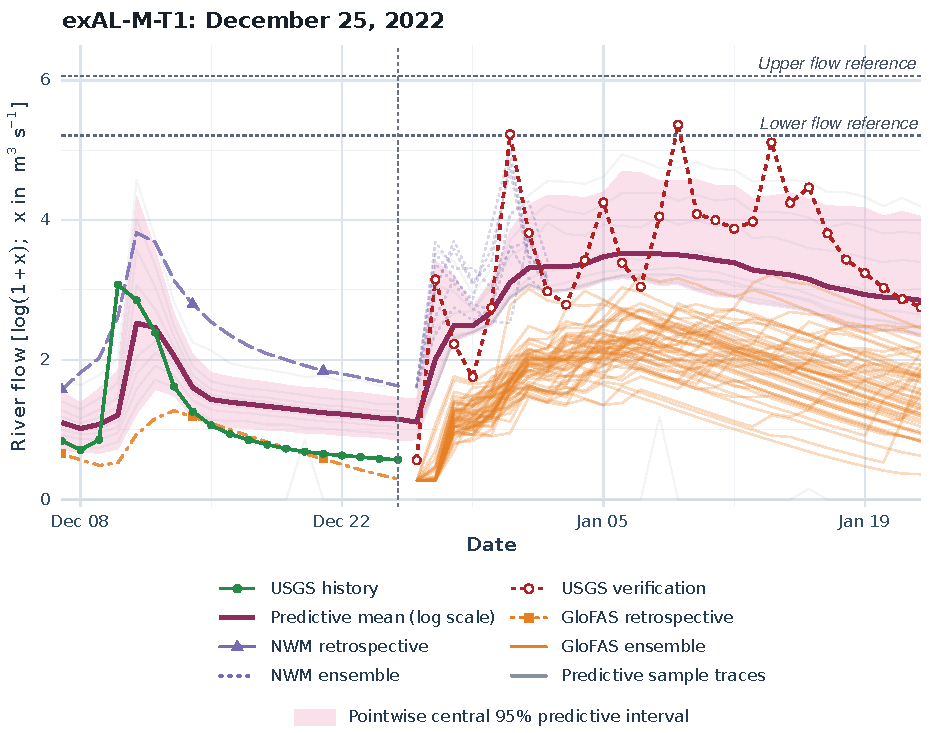
\includegraphics[width=450pt]{predictive_synthesis_2022_12_25.pdf}
\caption{Synthesized exAL-M-T1 prediction at December 25, 2022, on the $\log(1+x)$ scale, with $x$ in m$^3$/s. The 19 historical and 28 forecast dates show green historical observations and red open-circle verification values. The origin is $T$; the first lead is $T+1$. The maroon line is the predictive mean, the pink band is the pointwise central 95\% predictive interval (2.5th--97.5th percentiles), and ten gray traces connect predictive sample values within each period. Orange GloFAS and purple NWM products give source context; NWM denotes the NWS product family. Horizontal guides mark approximately 182 and 429~m$^3$/s. Figures~\ref{fig:forecast_origins_2021_early} and \ref{fig:forecast_origins_2021_2022} use the same conventions and vertical scale.}
\label{fig:synth1}
\end{figure}

\subsection{Distributional Forecast Performance}
\label{subsec:benchmarkresults}
\label{subsec:externalresults}

Table~\ref{tab:external_benchmarks} compares all nine Bayesian configurations and external references. The exAL-M-T1 mean-score reductions relative to climatology are 68.6\% over 28 days and 59.0\% over eight days. EMOS-GLOFAS also improves on climatology, with skill 0.288 and 0.391; persistence has negative skill at both horizons. Raw NWS is scored only over its eight available daily leads. Table~\ref{tab:crps_all_origins} reports every origin-specific comparison.

% Generated by scripts/compact_publication.py; edit the generator.
\begin{table}[!htbp]
\centering
\begin{threeparttable}
\caption{Mean forecast CRPS and skill relative to seasonal climatology across five origins.}
\label{tab:external_benchmarks}
\setlength{\tabcolsep}{4pt}
\begin{tabular}{lrrrr}
\hline
Method & 28-day CRPS & 28-day CRPSS & 8-day CRPS & 8-day CRPSS \\
\hline
N-U-T1 & 0.87008 & -0.35489 & 0.99005 & -0.35752 \\
N-M-T0 & 0.83948 & -0.30723 & 0.72381 & 0.00755 \\
N-M-T1 & 2.38126 & -2.70811 & 3.18134 & -3.36211 \\
AL-U-T1 & 0.60367 & 0.05997 & 0.34086 & 0.53263 \\
AL-M-T0 & 0.53820 & 0.16192 & 0.61368 & 0.15855 \\
AL-M-T1 & 0.23230 & 0.63826 & 0.30944 & 0.57570 \\
exAL-U-T1 & 0.59631 & 0.07143 & 0.35144 & 0.51812 \\
exAL-M-T0 & 1.13760 & -0.77147 & 1.13421 & -0.55518 \\
exAL-M-T1 & 0.20164 & 0.68601 & 0.29926 & 0.58967 \\
GloFAS & 0.61761 & 0.03826 & 0.77502 & -0.06267 \\
NWS & --- & --- & 0.66478 & 0.08848 \\
Seasonal climatology & 0.64218 & 0.00000 & 0.72931 & 0.00000 \\
Persistence & 0.91061 & -0.41801 & 0.99854 & -0.36915 \\
GloFAS EMOS & 0.45734 & 0.28782 & 0.44450 & 0.39052 \\
\hline
\end{tabular}
\begin{tablenotes}\footnotesize
\item \textit{Note:} Scores use $\log(1+x)$ discharge, with $x$ in m$^3$/s. CRPS denotes the continuous ranked probability score; lower values are better. CRPSS is one minus the ratio of pooled mean CRPS to the matching climatology mean; higher values are better. Means use 140 daily cases at leads 1--28 and 40 at leads 1--8. NWS has eight daily leads. Scores use quantile-grid integration. N, AL and exAL denote normal, asymmetric Laplace and extended asymmetric Laplace likelihoods; U and M denote one and multiple observation sources. T1 retains the transfer contribution at forecast leads and T0 omits it.
\end{tablenotes}
\end{threeparttable}
\end{table}


Within AL and exAL, source inclusion and retention of forecast transfer improve 28-day CRPS at every origin. The exAL-M-T1 model has the lowest score among the nine variants and raw products at all five origins. This is conditional on likelihood and horizon: N-M-T1 is worse than N-M-T0 at every origin over both horizons. Among the nine Bayesian variants and raw products over eight days, raw NWS has the lowest score in December 2021 and December 2022, AL-U-T1 in January 2021, and exAL-M-T1 in November 2021 and May 2022. Source inclusion improves exAL at four origins and AL at three; exAL-M-T1 improves on AL-M-T1 at four.

EMOS-GLOFAS outperforms exAL-M-T1 in May 2022: 28-day CRPS is 0.01763 versus 0.02273, and eight-day CRPS is 0.02381 versus 0.02567. The exAL-M-T1 model improves on all three benchmarks at the other four origins. Climatology itself outperforms EMOS in November 2021 (28-day scores 0.09588 versus 0.24060). Thus aggregate skill does not imply superiority at each origin. All 140 lead-specific EMOS fits satisfy optimizer convergence, using 143--364 training cases.

Exact empirical-distribution scores retain the principal aggregate transformed-scale ordering (Table~\ref{tab:exact_score_sensitivity}). For exAL-M-T1 they are 0.20156 and 0.29919, with skill 0.68602 and 0.58965. The independent-draw adjustment is small for 2,000-draw syntheses and larger for smaller Gaussian and raw ensembles. On the discharge scale (Table~\ref{tab:discharge_scale_scores}), exAL-M-T1 has 28-day CRPS 6.26885~m$^3$/s and skill 0.39113. Over eight days, raw NWS scores better, 6.63303 versus 7.49362~m$^3$/s, reversing their transformed-scale ordering. Large discharge-scale scores for N-M-T1 and exAL-M-T0 reveal extreme-tail sensitivity.

\subsection{Quantile Performance and Calibration}
\label{subsec:quantileresults}
\label{subsec:calibrationresults}

Table~\ref{tab:quantile_check_loss_pooled} summarizes 28-day check losses for four quantile-synthesis competitors; Table~\ref{tab:quantile_check_loss} gives the origin-specific results. Pooled exAL-M-T1 losses are smallest at probabilities 0.05--0.50, whereas AL-M-T1 is best at 0.65--0.95. Multivariate syntheses improve on univariate references in most origin--quantile cells. These targeted comparisons complement the distribution-wide CRPS.

% Generated by scripts/compact_publication.py; edit the generator.
\begin{table}[!htbp]
\centering
\begin{threeparttable}
\caption{Mean daily quantile check loss pooled over five 28-day forecast windows.}
\label{tab:quantile_check_loss_pooled}
\setlength{\tabcolsep}{4pt}
\begin{tabular}{lrrrrrrr}
\hline
Method & $0.05$ & $0.20$ & $0.35$ & $0.50$ & $0.65$ & $0.80$ & $0.95$ \\
\hline
AL-M-T1 & 0.04276 & 0.11409 & 0.15984 & 0.18053 & \textbf{0.13195} & \textbf{0.10446} & \textbf{0.05429} \\
AL-U-T1 & 0.05315 & 0.16341 & 0.25617 & 0.32472 & 0.39242 & 0.44899 & 0.46090 \\
exAL-M-T1 & \textbf{0.03057} & \textbf{0.07927} & \textbf{0.11265} & \textbf{0.14553} & 0.15261 & 0.10976 & 0.05582 \\
exAL-U-T1 & 0.04985 & 0.15945 & 0.25790 & 0.32564 & 0.38671 & 0.43920 & 0.45631 \\
\hline
\end{tabular}
\begin{tablenotes}\footnotesize
\item \textit{Note:} Columns are target probabilities; each entry averages 140 archived daily losses. Lower values are better; bold marks the minimum in each column. Scores use $\log(1+x)$ discharge, with $x$ in m$^3$/s. N, AL and exAL denote normal, asymmetric Laplace and extended asymmetric Laplace likelihoods; U and M denote one and multiple observation sources. T1 retains the transfer contribution at forecast leads and T0 omits it.
\end{tablenotes}
\end{threeparttable}
\end{table}


Individual exAL-M-T1 predictive quantiles cross on 61 of 140 forecast dates; neither their isotonic projection nor final synthesis crosses. Its mean check loss across seven probabilities decreases from 0.10058 to 0.09803 after synthesis over 28 days, and from 0.15069 to 0.14622 over eight days. Improvement is not universal: eight-day exAL-U-T1 loss increases from 0.17257 to 0.17259. Isotonic projection resolves crossings; synthesis can additionally change scores and calibration.

The exAL-M-T1 central 95\% interval covers 123/140 cases (87.86\%) over 28 days and 29/40 (72.50\%) over eight days (Table~\ref{tab:no_refit_calibration}). Eight-day coverage is 1/8 and 4/8 in December 2021 and December 2022, versus 8/8 at the other origins; the corresponding 28-day counts are 21/28 and 19/28 (Table~\ref{tab:origin_interval_coverage}). AL-M-T1 intervals are wider, cover 132/140 and 35/40 cases, and have lower mean interval scores. Favorable mean CRPS therefore coexists with undercoverage.

% Generated by scripts/compact_publication.py; edit the generator.
\begin{table}[!htbp]
\centering
\begin{threeparttable}
\caption{Coverage, mean width and mean interval score of central 95\% observation predictive intervals.}
\label{tab:no_refit_calibration}
\setlength{\tabcolsep}{4pt}
\begin{tabular}{lrrrrrr}
\hline
Method & \multicolumn{3}{c}{28 days} & \multicolumn{3}{c}{8 days} \\
 & Covered & Width & Interval score & Covered & Width & Interval score \\
\hline
exAL-M-T1 & 123/140 & 0.88870 & 2.50218 & 29/40 & 0.88509 & 4.46293 \\
AL-M-T1 & 132/140 & 1.45845 & \textbf{2.44957} & 35/40 & 1.55141 & \textbf{2.81501} \\
exAL-U-T1 & 75/140 & 0.62726 & 18.92775 & 27/40 & 0.79108 & 7.71508 \\
AL-U-T1 & 67/140 & 0.54957 & 19.49073 & 24/40 & 0.89059 & 6.83147 \\
GloFAS & 48/140 & 1.09584 & 15.64795 & 1/40 & 0.64042 & 23.02593 \\
NWS & --- & --- & --- & 12/40 & 0.64615 & 19.54956 \\
Seasonal climatology & 132/140 & 2.91666 & 4.28318 & 39/40 & 2.74092 & 4.14775 \\
Persistence & 0/140 & 0.00000 & 36.42450 & 0/40 & 0.00000 & 39.94145 \\
GloFAS EMOS & 106/140 & 1.63599 & 10.26329 & 27/40 & 1.70634 & 8.68153 \\
\hline
\end{tabular}
\begin{tablenotes}\footnotesize
\item \textit{Note:} Covered is the number of observations within the closed 2.5th--97.5th percentile interval divided by the case count. Width and interval score are averaged on the $\log(1+x)$ scale, with discharge $x$ in m$^3$/s. Bold marks the lowest interval score for each horizon. Persistence has zero width. Numerical quantile conventions are specified in Appendix~\ref{app:numericalprediction}. The monotone inverse transformation preserves coverage. N, AL and exAL denote normal, asymmetric Laplace and extended asymmetric Laplace likelihoods; U and M denote one and multiple observation sources. T1 retains the transfer contribution at forecast leads and T0 omits it.
\end{tablenotes}
\end{threeparttable}
\end{table}


Figure~\ref{fig:no_refit_reliability} shows quantile reliability. Over 28 days, exAL-M-T1 strict frequencies at 0.05, 0.50 and 0.95 are 6/140, 67/140 and 128/140. The upper frequency is below nominal, consistent with upper-tail misses; complete counts and ties accompany the reproducibility materials.

\begin{figure}[!htbp]
\centering
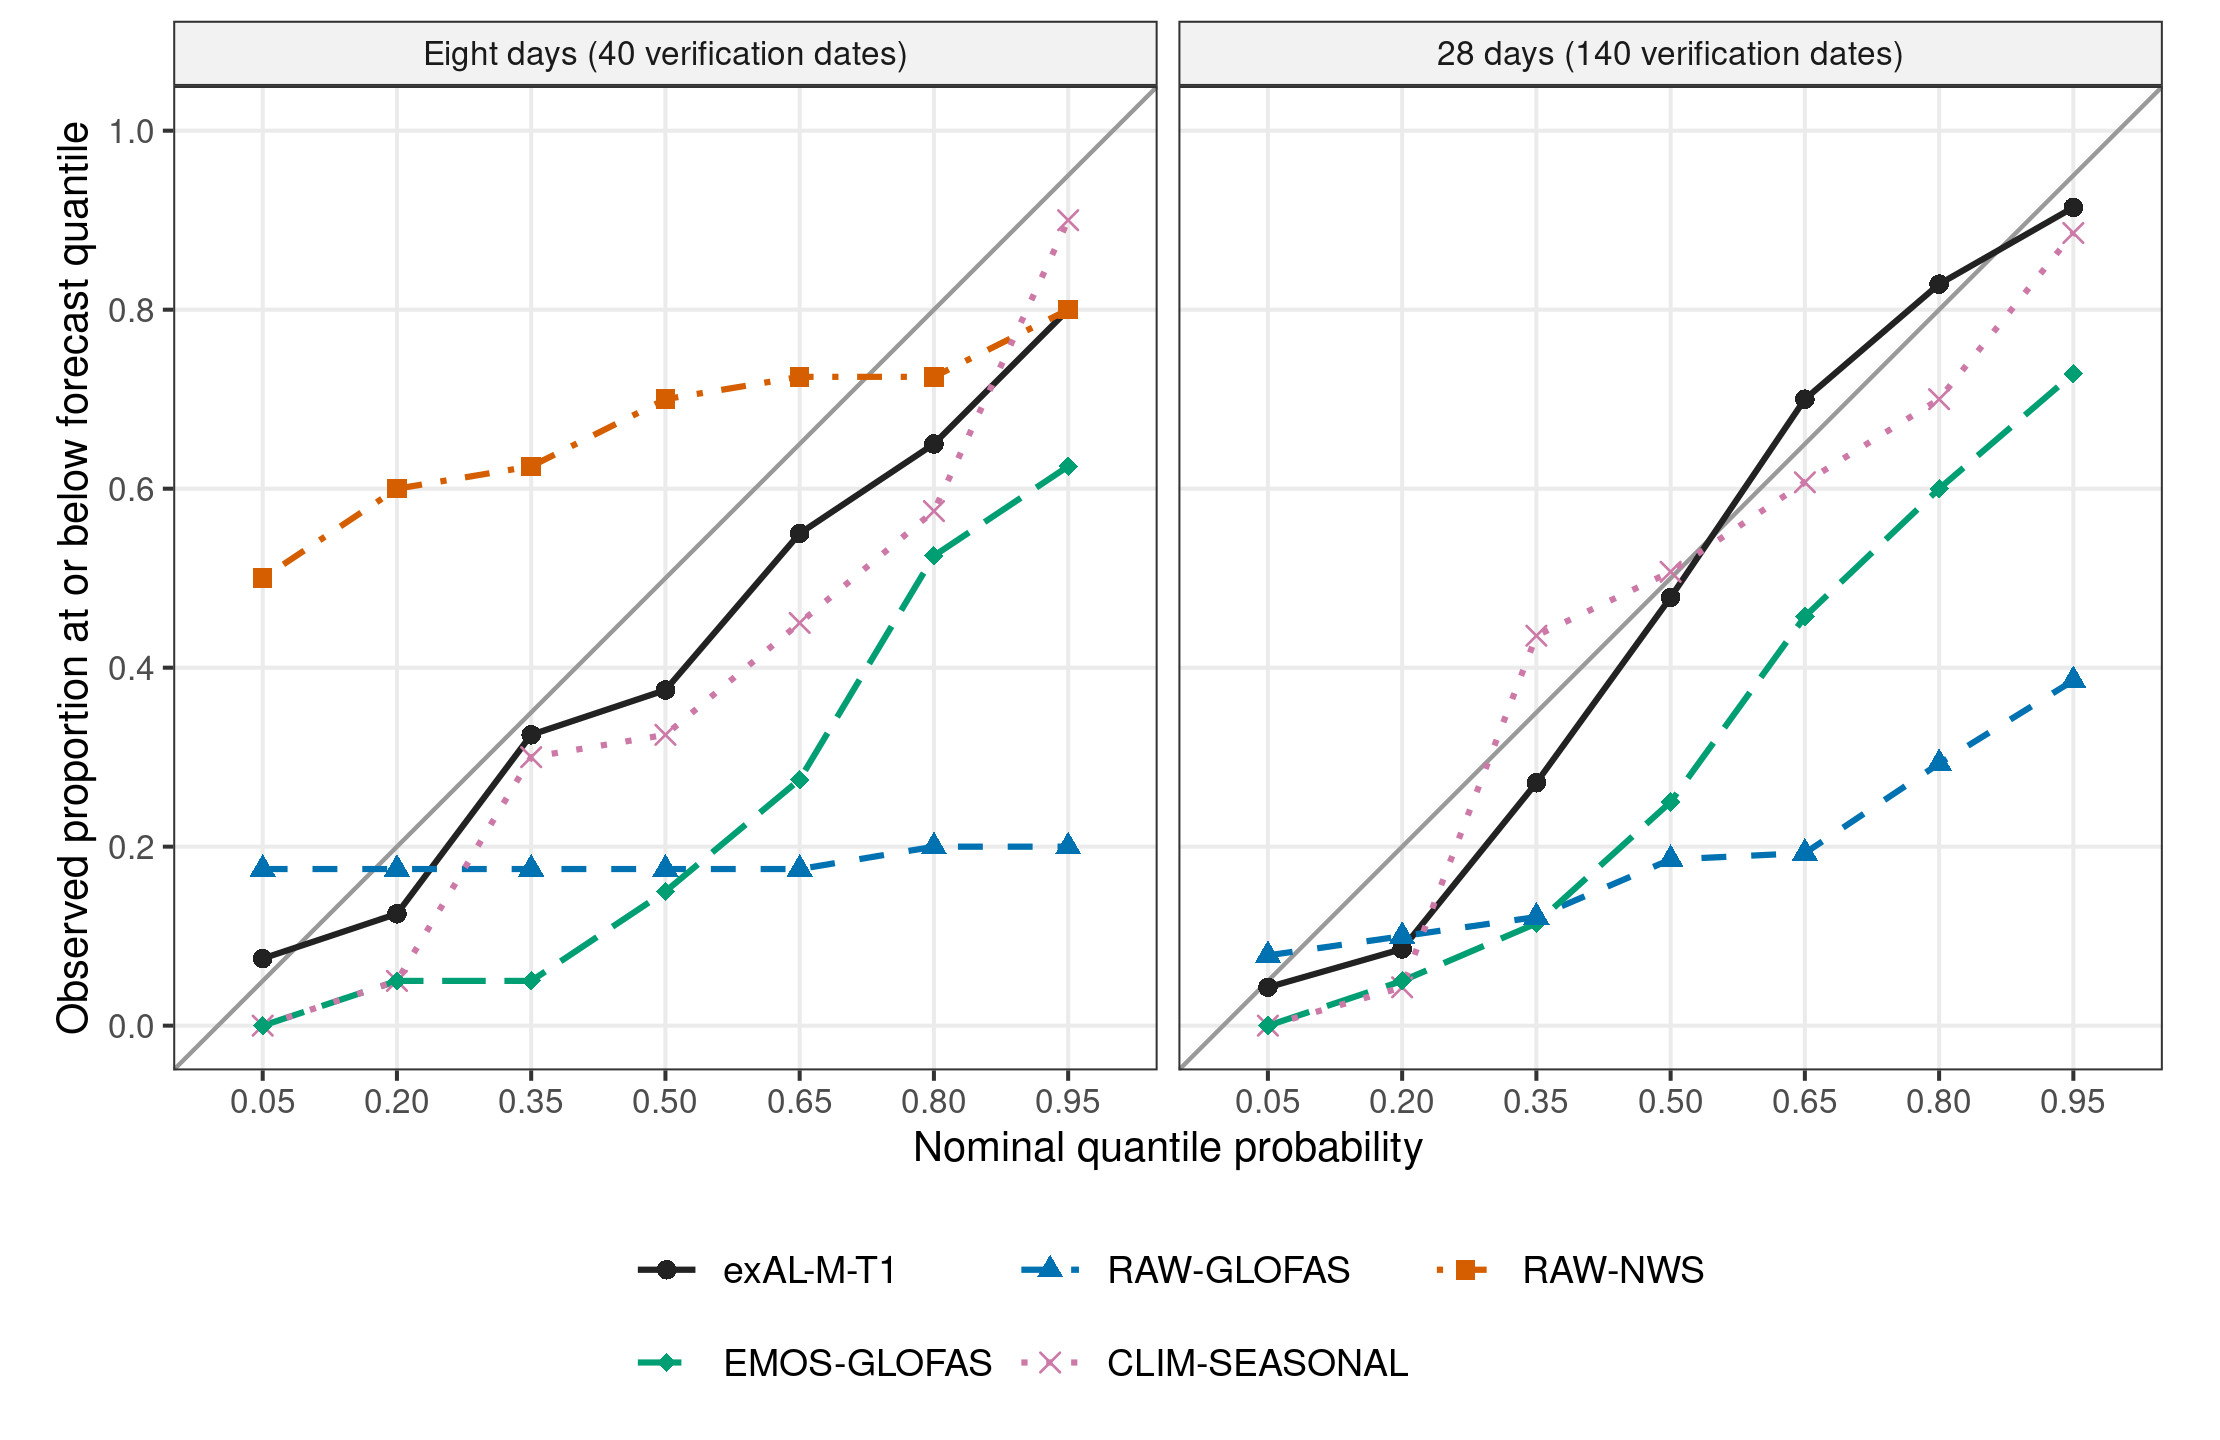
\includegraphics[width=450pt]{no_refit_quantile_reliability.png}
\caption{Quantile reliability over eight and 28 days, pooling 40 and 140 cases across five origins. Curves give frequencies at or below predictive quantiles for exAL-M-T1, raw GloFAS/NWS, EMOS-GLOFAS and seasonal climatology; the diagonal denotes nominal probabilities. NWS is available over eight days. Strict frequencies and ties are retained in the reproducibility materials.}
\label{fig:no_refit_reliability}
\end{figure}

\subsection{Component Sensitivity and Interpretation}
\label{subsec:componentresults}
\label{sec:interpretation}

Each one-component reduction has higher CRPS than the full exAL-M-T1 reference and raw GloFAS at every origin over both horizons (Table~\ref{tab:component_comparison}). The reductions illustrate sensitivity to model structure under common fitting settings. In May 2022, the transfer-free fitted median locations range from 10.53 to 10.81 against transformed verification values of 0.42--0.57.

Table~\ref{tab:components_23_31} reports terminal coefficient states $\boldsymbol\psi_T$ for the three base inputs at December 25, 2022, per historical-standard-deviation unit. Their signs describe conditional adjustments alongside source products, discrepancies, seasonality, nonlinear terms and lags. A negative linear precipitation coefficient does not imply that rainfall reduces total flow: the complete covariate vector and persistent transfer state determine the adjustment. Coefficients have no causal interpretation. Their central 95\% variational credible intervals summarize parameter uncertainty under the approximate posterior; mean-field and local Laplace--Delta approximations can omit posterior dependence \citep{blei2017variational}. A predictive interval instead concerns a future discharge observation, combining parameter and latent-state uncertainty with observation variation and, here, synthesis across quantile-specific predictive distributions. Predictive agreement or coverage does not establish accurate parameter credible intervals, and parameter accuracy alone does not guarantee predictive calibration.

\section{DISCUSSION AND CONCLUSIONS}
\label{sec5}

A shared dynamic quantile process corrects external products through source-specific discrepancies while accommodating different forecast horizons. Predictive synthesis uses the full distributions from separate quantile fits, including their tails, to construct a nondecreasing marginal quantile function. Joint scale--skewness updates through model-specific Laplace--Delta VB make the extended-likelihood analysis practical for a long daily record.

The principal empirical gain is 28-day distributional prediction in the San Lorenzo comparisons. The exAL-M-T1 specification reduces mean transformed-scale CRPS by 67.4\% relative to raw GloFAS and 55.9\% relative to GloFAS EMOS. It outperforms the other Bayesian variants at every origin and EMOS at four of five origins; its aggregate 28-day advantage also persists on the discharge scale. EMOS performs better in May 2022 over both horizons, whereas raw NWS leads at the two winter eight-day origins. AL-M-T1 has smaller pooled upper-quantile losses, better interval coverage and a lower aggregate eight-day discharge-scale score than exAL-M-T1. These comparisons identify the horizons and forecast characteristics for which the fuller construction is most useful.

Predictive scores and calibration provide complementary assessments. Favorable transformed-scale CRPS coexists with December undercoverage, and raw NWS also improves on the reference's aggregate eight-day discharge-scale score. The likelihood assumes independent residual member contributions given the states and shares source scales across leads. Parameter credible intervals and predictive intervals describe different uncertainties; predictive performance does not establish posterior approximation accuracy.

The method depends on aligned external products and supplied covariate paths. A denser evaluation requires a larger version-consistent historical archive. A controlled simulation study could compare VB and MCMC for matching models and manageable data sizes, then apply identical predictive synthesis to both sets of predictive draws. Parameter accuracy, predictive agreement and interval coverage across independent simulated datasets would be assessed separately. Further work could also propagate transfer-input uncertainty, model dependent quantiles jointly, enrich discrepancies and extend the method to multiple sites.

\section*{Acknowledgments}
This work forms part of Antonio De Leon's Ph.D. dissertation in statistical science at the University of California, Santa Cruz.

\section*{Funding Statement}
Supported in part by National Science Foundation grant MMS2050012.

\section*{Conflict of Interest Statement}
The authors declare no conflict of interest.

\section*{Data Availability Statement}
Analysis data, data-source documentation, statistical code and numerical results are available in the public reproducibility repository \citep{deleon2026sanlorenzo_reproducibility}. Public source products are described in Section~\ref{sec:data} and Appendix~\ref{app:datahistories}.

\section*{Code availability}
The R package \texttt{exdqlm}, version 1.1.0, provides estimation routines on the Comprehensive R Archive Network (CRAN; \url{https://CRAN.R-project.org/package=exdqlm}; DOI \url{https://doi.org/10.32614/CRAN.package.exdqlm}; \citealp{deleon2026exdqlm}). The reproducibility materials supply the analysis code for fits, scores, tables and figures. A new application requires corresponding observations, products and covariates; retrospective evaluation also requires a version-consistent forecast archive.

% The Wiley class provides the appendix environment and lettered sections.
% Reset exhibit counters within each appendix and keep hyperlink targets unique.
\FloatBarrier
\begin{appendix}
\makeatletter
\@addtoreset{figure}{section}
\@addtoreset{table}{section}
\@addtoreset{equation}{section}
\@addtoreset{algorithm}{section}
\makeatother
\renewcommand{\thefigure}{\Alph{section}\arabic{figure}}
\renewcommand{\thetable}{\Alph{section}\arabic{table}}
\renewcommand{\theequation}{\Alph{section}\arabic{equation}}
\renewcommand{\thealgorithm}{\Alph{section}\arabic{algorithm}}
\renewcommand{\theHfigure}{appendix.\Alph{section}.\arabic{figure}}
\renewcommand{\theHtable}{appendix.\Alph{section}.\arabic{table}}
\renewcommand{\theHequation}{appendix.\Alph{section}.\arabic{equation}}
\providecommand{\theHalgorithm}{}
\renewcommand{\theHalgorithm}{appendix.\Alph{section}.\arabic{algorithm}}
\section{Data Sources and Historical Inputs}
\label{app:datahistories}

The target is daily mean discharge at the U.S. Geological Survey (USGS) Big Trees gauge, station 11160500, Santa Cruz, California \citep{usgs_daily_11160500}. The 12,995-observation record spans May 29, 1987 through December 25, 2022. Figures~\ref{fig:covariates} and \ref{fig:retrospectives} display the historical covariates and retrospective products. All modeled discharge is transformed as $\log(1+x)$, with $x$ in m$^3$/s. A forecast origin $T$ ends the historical window; verification starts at $T+1$.

The base covariates are precipitation from the Parameter-elevation Regressions on Independent Slopes Model (PRISM) Climate Group \citep{prism}, soil moisture from European Centre for Medium-Range Weather Forecasts (ECMWF) ERA5-Land \citep{ecmwf,munozsabater2021era5land}, and a generalized dynamic principal component (GDPC; \citealp{JSSv092c02}) of National Oceanic and Atmospheric Administration (NOAA) Physical Sciences Laboratory climate indices \citep{noaa_climate_indices}. The monthly indices are solar flux, Ni\~no 1+2, Oceanic Ni\~no Index, Southern Oscillation Index, Western Hemisphere Warm Pool, global mean temperature, Northern Oscillation Index, Atlantic Multidecadal Oscillation, and tropical South and North Atlantic indices. They are interpolated to daily resolution and standardized; the first GDPC explains 44.07\% of total variability. Forecast covariate paths include Global Ensemble Forecast System precipitation and shallow soil water.

External discharge comes from ECMWF's Global Flood Awareness System (GloFAS; \citealp{harrigan2020glofas}) and NOAA National Weather Service (NWS), including National Water Model (NWM) output \citep{cosgrove2024noaa}. Gridded covariates and GloFAS use the gauge cell or nearest valid river cell; NWM uses the corresponding reach or model-output point. PRISM has 4 km resolution and ERA5-Land 0.1-degree resolution. GloFAS retrospective version 2.1 is used for January 2021 and version 3.1 for other origins; NWM version 2.1 has a version 3.0 extension beyond its coverage. Hourly NWS forecasts retain the latest available issuance for each target and member at the origin before daily aggregation. GloFAS contributes 51 members over 28 daily leads and NWS seven members over eight valid daily leads. Data-source records document extraction and versions by origin \citep{deleon2026sanlorenzo_reproducibility}.

\begin{figure}[!htbp]
\centering
\includegraphics[width=450pt]{covariate_context_precip_soil_gdpc.png}
\caption{Historical daily precipitation (mm), soil moisture (m$^3$/m$^3$) and first GDPC score, May 29, 1987 through December 25, 2022.}
\label{fig:covariates}
\end{figure}

\begin{figure}[!htbp]
\centering
\includegraphics[width=450pt]{retrospective_products_context.png}
\caption{GloFAS and NWS retrospective discharge over available coverage for the December 25, 2022 origin. Values are on the $\log(1+x)$ scale with $x$ in m$^3$/s; the displayed record spans May 29, 1987 through December 25, 2022.}
\label{fig:retrospectives}
\end{figure}

\section{Additional Forecast Results}
\label{app:extras}

\subsection{Model Comparisons by Origin}
\label{app:externalreferences}

The five origins are January 23, November 12 and December 21, 2021, and May 11 and December 25, 2022. Nine Bayesian variants combine Gaussian (N), asymmetric Laplace (AL) or extended asymmetric Laplace (exAL) likelihoods with gauge-only (U) or source-inclusive (M) observations and transfer-active (T1) or forecast-transfer-suppressed (T0) configurations. M-T0 retains transfer during historical fitting. AL/exAL predictive syntheses combine fits at probabilities $0.05,0.20,0.35,0.50,0.65,0.80,0.95$. The exAL-M-T1 configuration is the reference specification.

Table~\ref{tab:crps_all_origins} gives mean continuous ranked probability scores (CRPS; smaller is better) using the reported quantile-grid calculation on transformed discharge. External references are raw GloFAS/NWS ensembles, seasonal climatology, persistence and GloFAS ensemble model output statistics (EMOS). The horizons retain matching verification dates, with NWS available only for eight days. Aggregate means and climatology-relative skill appear in Table~\ref{tab:external_benchmarks}.

% Generated by scripts/compact_publication.py; edit the generator.
\begin{table}[!htbp]
\centering
\begin{threeparttable}
\caption{Mean quantile-grid CRPS by forecast origin and horizon.}
\label{tab:crps_all_origins}
\setlength{\tabcolsep}{4pt}
\begin{tabular}{lrrrrr}
\hline
Method & Jan 2021 & Nov 2021 & Dec 2021 & May 2022 & Dec 2022 \\
\hline
% horizon_days=28
\multicolumn{6}{l}{\textit{28-day horizon}} \\
N-U-T1 & 0.33592 & 0.17059 & 1.19344 & 0.15077 & 2.49968 \\
N-M-T0 & 1.84333 & 0.38023 & 0.65964 & 0.67014 & 0.64404 \\
N-M-T1 & 3.21490 & 0.89096 & 3.04362 & 0.86820 & 3.88863 \\
AL-U-T1 & 0.23107 & 0.07795 & 0.87049 & 0.10506 & 1.73376 \\
AL-M-T0 & 0.46798 & 0.19990 & 0.58668 & 0.09940 & 1.33703 \\
AL-M-T1 & 0.14592 & 0.05551 & 0.27775 & 0.05467 & 0.62764 \\
exAL-U-T1 & 0.21622 & 0.10194 & 0.83337 & 0.12452 & 1.70548 \\
exAL-M-T0 & 0.75682 & 1.72135 & 0.97762 & 1.02087 & 1.21132 \\
exAL-M-T1 & 0.13971 & 0.04724 & 0.26045 & 0.02273 & 0.53806 \\
GloFAS & 0.40366 & 0.16957 & 0.68246 & 0.27227 & 1.56006 \\
Seasonal climatology & 0.45262 & 0.09588 & 0.79703 & 0.15235 & 1.71301 \\
Persistence & 0.62063 & 0.22551 & 0.69663 & 0.09059 & 2.91971 \\
GloFAS EMOS & 0.26847 & 0.24060 & 0.45633 & 0.01763 & 1.30369 \\
\hline
% horizon_days=8
\multicolumn{6}{l}{\textit{8-day horizon}} \\
N-U-T1 & 0.76838 & 0.13732 & 2.04040 & 0.12611 & 1.87805 \\
N-M-T0 & 1.31032 & 0.25581 & 0.41461 & 0.63732 & 1.00096 \\
N-M-T1 & 4.72798 & 0.71930 & 5.13027 & 0.79737 & 4.53177 \\
AL-U-T1 & 0.18835 & 0.10367 & 0.75625 & 0.03599 & 0.62002 \\
AL-M-T0 & 0.63929 & 0.16893 & 1.15588 & 0.09506 & 1.00922 \\
AL-M-T1 & 0.23740 & 0.07170 & 0.56351 & 0.05867 & 0.61593 \\
exAL-U-T1 & 0.18999 & 0.11312 & 0.77939 & 0.04489 & 0.62982 \\
exAL-M-T0 & 0.94687 & 1.69464 & 0.69022 & 1.02364 & 1.31568 \\
exAL-M-T1 & 0.22691 & 0.05858 & 0.59445 & 0.02567 & 0.59070 \\
GloFAS & 0.57251 & 0.20670 & 1.29127 & 0.32274 & 1.48188 \\
NWS & 0.83037 & 1.37192 & 0.28118 & 0.28366 & 0.55680 \\
Seasonal climatology & 0.56808 & 0.06898 & 1.49136 & 0.16292 & 1.35522 \\
Persistence & 1.09161 & 0.15108 & 1.47804 & 0.03160 & 2.24035 \\
GloFAS EMOS & 0.64070 & 0.11361 & 0.64016 & 0.02381 & 0.80423 \\
\hline
\end{tabular}
\begin{tablenotes}\footnotesize
\item \textit{Note:} Scores use $\log(1+x)$ discharge, with $x$ in m$^3$/s. Each entry averages the stated number of daily leads; lower is better. Origins are January 23, November 12 and December 21, 2021, and May 11 and December 25, 2022. NWS has only eight daily leads. N, AL and exAL denote normal, asymmetric Laplace and extended asymmetric Laplace likelihoods; U and M denote one and multiple observation sources. T1 retains the transfer contribution at forecast leads and T0 omits it.
\end{tablenotes}
\end{threeparttable}
\end{table}


\subsection{Component-Removal Comparisons}
\label{app:he3ablation}

The reductions retain reference settings while removing one structural component. The labels \texttt{noTrend}, \texttt{noH1}, \texttt{noH2} and \texttt{noH3} remove the shared and source-discrepancy local level or corresponding seasonal pair. The third pair has period 2474.87 days (Subsection~\ref{app:seasonalconstruction}). The \texttt{noTF} model removes transfer in both fitting and forecasting, unlike T0. Table~\ref{tab:component_comparison} gives the comparisons over both horizons and all five origins.

% Generated by scripts/compact_publication.py; edit the generator.
\begin{table}[!htbp]
\centering
\begin{threeparttable}
\caption{Mean CRPS for the full exAL-M-T1 model and component-removal comparisons.}
\label{tab:component_comparison}
\setlength{\tabcolsep}{4pt}
\begin{tabular}{lrrrrr}
\hline
Method & Jan 2021 & Nov 2021 & Dec 2021 & May 2022 & Dec 2022 \\
\hline
% horizon_days=28
\multicolumn{6}{l}{\textit{28-day horizon}} \\
GloFAS & 0.40366 & 0.16957 & 0.68246 & 0.27227 & 1.56006 \\
exAL-M-T1 (full) & \textbf{0.13971} & \textbf{0.04724} & \textbf{0.26045} & \textbf{0.02273} & \textbf{0.53806} \\
exAL-M-T1-noTrend & 1.05159 & 0.72343 & 2.51748 & 0.53257 & 4.05881 \\
exAL-M-noTF & 1.73610 & 1.71409 & 2.32863 & 2.47703 & 2.17280 \\
exAL-M-T1-noH1 & 1.27861 & 1.60142 & 2.83017 & 1.09956 & 4.45887 \\
exAL-M-T1-noH2 & 0.72690 & 1.04699 & 2.96513 & 0.91193 & 4.64709 \\
exAL-M-T1-noH3 & 1.08281 & 1.03562 & 2.58333 & 0.68642 & 4.43879 \\
\hline
% horizon_days=8
\multicolumn{6}{l}{\textit{8-day horizon}} \\
GloFAS & 0.57251 & 0.20670 & 1.29127 & 0.32274 & 1.48188 \\
NWS & 0.83037 & 1.37192 & \textbf{0.28118} & 0.28366 & \textbf{0.55680} \\
exAL-M-T1 (full) & \textbf{0.22691} & \textbf{0.05858} & 0.59445 & \textbf{0.02567} & 0.59070 \\
exAL-M-T1-noTrend & 1.49490 & 0.77464 & 3.38697 & 0.64627 & 3.40333 \\
exAL-M-noTF & 1.79777 & 1.69066 & 2.18697 & 2.45857 & 2.30863 \\
exAL-M-T1-noH1 & 1.66963 & 1.69424 & 3.70227 & 1.14270 & 3.79228 \\
exAL-M-T1-noH2 & 1.11122 & 1.14286 & 3.80753 & 0.99851 & 3.92807 \\
exAL-M-T1-noH3 & 1.53419 & 1.09181 & 3.45450 & 0.78219 & 3.75262 \\
\hline
\end{tabular}
\begin{tablenotes}\footnotesize
\item \textit{Note:} Scores use $\log(1+x)$ discharge, with $x$ in m$^3$/s. Scores use quantile-grid integration and the five origins listed in Table~\ref{tab:crps_all_origins}. Suffixes noTrend, noTF and noH1--noH3 remove the trend, transfer component and respective harmonic blocks. Structural removal of the transfer component differs from T0, which omits its forecast contribution. GloFAS and NWS are uncorrected references; NWS has eight leads. Bold marks the lowest CRPS in each origin column within each horizon.
\end{tablenotes}
\end{threeparttable}
\end{table}


\subsection{Quantile Loss and Distributional Diagnostics}
\label{app:distributionchecks}

Table~\ref{tab:quantile_check_loss} reports check losses for each origin and target probability; Table~\ref{tab:quantile_check_loss_pooled} gives the pooled 28-day comparison. These are losses of synthesized predictive quantiles against subsequent USGS observations, not losses of conditional model locations. Tables~\ref{tab:exact_score_sensitivity} and \ref{tab:discharge_scale_scores} distinguish exact empirical-distribution scores, the independent-draw sensitivity and discharge-scale results. Subsection~\ref{app:numericalprediction} defines their finite-representation conventions. Table~\ref{tab:origin_interval_coverage} reports the origin-specific central 95\% interval counts. The analysis materials also provide complete reliability hits, ties, interval scores and raw-product error/spread summaries \citep{deleon2026sanlorenzo_reproducibility}.

% Generated by scripts/compact_publication.py; edit the generator.
\begin{table}[!htbp]
\centering
\begin{threeparttable}
\caption{Mean daily quantile check loss by forecast origin and probability.}
\label{tab:quantile_check_loss}
\setlength{\tabcolsep}{4pt}
\begin{tabular}{lrrrrrrr}
\hline
Method & $0.05$ & $0.20$ & $0.35$ & $0.50$ & $0.65$ & $0.80$ & $0.95$ \\
\hline
% Origin 01/23/2021
\multicolumn{8}{l}{\textit{January 23, 2021}} \\
AL-M-T1 & 0.02894 & 0.07178 & 0.09341 & 0.09700 & 0.08931 & 0.06937 & 0.04116 \\
AL-U-T1 & 0.03150 & 0.08874 & 0.12511 & 0.13534 & 0.14456 & 0.14617 & 0.12576 \\
exAL-M-T1 & 0.02529 & 0.07061 & 0.09149 & 0.09407 & 0.08697 & 0.07165 & 0.03093 \\
exAL-U-T1 & 0.03314 & 0.09434 & 0.12252 & 0.13140 & 0.13265 & 0.12867 & 0.10144 \\
% Origin 11/12/2021
\multicolumn{8}{l}{\textit{November 12, 2021}} \\
AL-M-T1 & 0.01114 & 0.02242 & 0.02264 & 0.03547 & 0.03937 & 0.03394 & 0.02369 \\
AL-U-T1 & 0.01843 & 0.02075 & 0.07354 & 0.06746 & 0.04860 & 0.02874 & 0.01018 \\
exAL-M-T1 & 0.00943 & 0.02226 & 0.02164 & 0.03224 & 0.03659 & 0.02737 & 0.01267 \\
exAL-U-T1 & 0.01110 & 0.02586 & 0.08966 & 0.09603 & 0.06947 & 0.04183 & 0.01279 \\
% Origin 12/21/2021
\multicolumn{8}{l}{\textit{December 21, 2021}} \\
AL-M-T1 & 0.05594 & 0.10246 & 0.14994 & 0.17786 & 0.22531 & 0.17118 & 0.05205 \\
AL-U-T1 & 0.06384 & 0.23665 & 0.33938 & 0.45254 & 0.57593 & 0.67517 & 0.68584 \\
exAL-M-T1 & 0.02204 & 0.08243 & 0.13306 & 0.17423 & 0.21136 & 0.17833 & 0.08278 \\
exAL-U-T1 & 0.06544 & 0.22311 & 0.33019 & 0.42750 & 0.54414 & 0.64406 & 0.67338 \\
% Origin 05/11/2022
\multicolumn{8}{l}{\textit{May 11, 2022}} \\
AL-M-T1 & 0.01095 & 0.03552 & 0.03957 & 0.03433 & 0.02135 & 0.02730 & 0.01661 \\
AL-U-T1 & 0.03186 & 0.03619 & 0.09686 & 0.08487 & 0.06068 & 0.03675 & 0.01363 \\
exAL-M-T1 & 0.00754 & 0.00818 & 0.00784 & 0.01526 & 0.01387 & 0.01399 & 0.00904 \\
exAL-U-T1 & 0.01852 & 0.04289 & 0.10852 & 0.10902 & 0.07885 & 0.04803 & 0.01501 \\
% Origin 12/25/2022
\multicolumn{8}{l}{\textit{December 25, 2022}} \\
AL-M-T1 & 0.10685 & 0.33826 & 0.49367 & 0.55801 & 0.28439 & 0.22049 & 0.13795 \\
AL-U-T1 & 0.12012 & 0.43475 & 0.64594 & 0.88340 & 1.13232 & 1.35815 & 1.46909 \\
exAL-M-T1 & 0.08853 & 0.21289 & 0.30922 & 0.41184 & 0.41426 & 0.25746 & 0.14369 \\
exAL-U-T1 & 0.12106 & 0.41104 & 0.63858 & 0.86423 & 1.10845 & 1.33342 & 1.47893 \\
\hline
\end{tabular}
\begin{tablenotes}\footnotesize
\item \textit{Note:} Each entry averages 28 archived daily losses at the column probability. Lower values are better. Scores use $\log(1+x)$ discharge, with $x$ in m$^3$/s. N, AL and exAL denote normal, asymmetric Laplace and extended asymmetric Laplace likelihoods; U and M denote one and multiple observation sources. T1 retains the transfer contribution at forecast leads and T0 omits it.
\end{tablenotes}
\end{threeparttable}
\end{table}

% Generated by scripts/compact_publication.py; edit the generator.
\begin{table}[!htbp]
\centering
\begin{threeparttable}
\caption{Exact empirical-distribution scores and independent-draw sensitivity.}
\label{tab:exact_score_sensitivity}
\setlength{\tabcolsep}{4pt}
\begin{tabular}{lrrr}
\hline
Method & Exact CRPS & CRPSS & Adjusted CRPS \\
\hline
% horizon_days=28
\multicolumn{4}{l}{\textit{28-day horizon}} \\
N-U-T1 & 0.86656 & -0.34986 & 0.86294 \\
N-M-T0 & 0.83341 & -0.29821 & 0.82708 \\
N-M-T1 & 2.37057 & -2.69267 & 2.35942 \\
AL-U-T1 & 0.60362 & 0.05973 & 0.60358 \\
AL-M-T0 & 0.53804 & 0.16189 & 0.53788 \\
AL-M-T1 & 0.23218 & 0.63833 & 0.23206 \\
exAL-U-T1 & 0.59626 & 0.07120 & 0.59621 \\
exAL-M-T0 & 1.13635 & -0.77011 & 1.13511 \\
exAL-M-T1 & 0.20156 & 0.68602 & 0.20149 \\
GloFAS & 0.61456 & 0.04269 & 0.61139 \\
Seasonal climatology & 0.64197 & 0.00000 & --- \\
Persistence & 0.91061 & -0.41847 & --- \\
GloFAS EMOS & 0.45722 & 0.28778 & --- \\
\hline
% horizon_days=8
\multicolumn{4}{l}{\textit{8-day horizon}} \\
N-U-T1 & 0.98660 & -0.35315 & 0.98304 \\
N-M-T0 & 0.71763 & 0.01575 & 0.71119 \\
N-M-T1 & 3.16734 & -3.34409 & 3.15275 \\
AL-U-T1 & 0.34079 & 0.53260 & 0.34072 \\
AL-M-T0 & 0.61352 & 0.15854 & 0.61336 \\
AL-M-T1 & 0.30932 & 0.57576 & 0.30920 \\
exAL-U-T1 & 0.35138 & 0.51807 & 0.35132 \\
exAL-M-T0 & 1.13298 & -0.55391 & 1.13174 \\
exAL-M-T1 & 0.29919 & 0.58965 & 0.29912 \\
GloFAS & 0.77322 & -0.06048 & 0.77134 \\
NWS & 0.65025 & 0.10817 & 0.63086 \\
Seasonal climatology & 0.72911 & 0.00000 & --- \\
Persistence & 0.99854 & -0.36952 & --- \\
GloFAS EMOS & 0.44438 & 0.39053 & --- \\
\hline
\end{tabular}
\begin{tablenotes}\footnotesize
\item \textit{Note:} Scores use $\log(1+x)$ discharge, with $x$ in m$^3$/s. Exact CRPS gives equal weight to each predictive sample or grid value; CRPSS uses the matching exact climatology score. Means pool 140 or 40 cases. Adjusted CRPS applies the pairwise correction for independent, identically distributed predictive draws. Independence of physical ensemble members is a sensitivity assumption. Counts are 2,000 for AL/exAL, 64 for N-U-T1, 48 for N-M-T0/T1, 51 for GloFAS and seven for NWS. The adjustment is inapplicable to deterministic climatology and EMOS grids and to persistence; dashes denote this inapplicability. Adjusted skill is not reported. N, AL and exAL denote normal, asymmetric Laplace and extended asymmetric Laplace likelihoods; U and M denote one and multiple observation sources. T1 retains the transfer contribution at forecast leads and T0 omits it.
\end{tablenotes}
\end{threeparttable}
\end{table}

% Generated by scripts/compact_publication.py; edit the generator.
\begin{table}[!htbp]
\centering
\begin{threeparttable}
\caption{Exact empirical-distribution forecast scores on the discharge scale.}
\label{tab:discharge_scale_scores}
\setlength{\tabcolsep}{4pt}
\begin{tabular}{lrrrr}
\hline
Method & 28-day CRPS & 28-day CRPSS & 8-day CRPS & 8-day CRPSS \\
\hline
N-U-T1 & 11.92540 & -0.15827 & 12.37612 & -0.17558 \\
N-M-T0 & 10.95380 & -0.06390 & 9.97545 & 0.05245 \\
N-M-T1 & $2.03084\times 10^{9}$ & $-1.97248\times 10^{8}$ & $7.10790\times 10^{9}$ & $-6.75163\times 10^{8}$ \\
AL-U-T1 & 10.25614 & 0.00386 & 7.74218 & 0.26459 \\
AL-M-T0 & 10.13001 & 0.01611 & 10.42987 & 0.00929 \\
AL-M-T1 & 6.34032 & 0.38419 & 7.37167 & 0.29978 \\
exAL-U-T1 & 10.27183 & 0.00234 & 7.92688 & 0.24704 \\
exAL-M-T0 & 12307.63341 & -1194.39488 & 5460.23472 & -517.65541 \\
exAL-M-T1 & 6.26885 & 0.39113 & 7.49362 & 0.28820 \\
GloFAS & 10.67159 & -0.03649 & 11.31853 & -0.07512 \\
NWS & --- & --- & 6.63303 & 0.36994 \\
Seasonal climatology & 10.29587 & 0.00000 & 10.52767 & 0.00000 \\
Persistence & 11.98266 & -0.16383 & 12.37425 & -0.17540 \\
GloFAS EMOS & 9.59933 & 0.06765 & 9.03252 & 0.14202 \\
\hline
\end{tabular}
\begin{tablenotes}\footnotesize
\item \textit{Note:} Each predictive value is transformed by $\exp(y)-1$ before scoring; transformed-scale scores are not exponentiated. CRPS is in m$^3$/s and CRPSS is dimensionless. The empirical distribution weights each sample or grid value equally. Skill uses matching seasonal-climatology scores. Means pool 140 or 40 daily cases; NWS has eight leads. N, AL and exAL denote normal, asymmetric Laplace and extended asymmetric Laplace likelihoods; U and M denote one and multiple observation sources. T1 retains the transfer contribution at forecast leads and T0 omits it.
\end{tablenotes}
\end{threeparttable}
\end{table}

% Generated by scripts/compact_publication.py; edit the generator.
\begin{table}[!htbp]
\centering
\begin{threeparttable}
\caption{Central 95\% observation predictive interval coverage by origin and horizon.}
\label{tab:origin_interval_coverage}
\setlength{\tabcolsep}{4pt}
\begin{tabular}{lrrrrr}
\hline
Method & Jan 2021 & Nov 2021 & Dec 2021 & May 2022 & Dec 2022 \\
\hline
% horizon_days=28
\multicolumn{6}{l}{\textit{28-day horizon}} \\
N-U-T1 & 26/28 & 28/28 & 12/28 & 28/28 & 3/28 \\
N-M-T0 & 3/28 & 6/28 & 17/28 & 1/28 & 24/28 \\
N-M-T1 & 0/28 & 0/28 & 0/28 & 0/28 & 2/28 \\
AL-U-T1 & 15/28 & 20/28 & 5/28 & 24/28 & 3/28 \\
AL-M-T0 & 25/28 & 28/28 & 17/28 & 28/28 & 3/28 \\
AL-M-T1 & 28/28 & 28/28 & 26/28 & 27/28 & 23/28 \\
exAL-U-T1 & 17/28 & 27/28 & 2/28 & 26/28 & 3/28 \\
exAL-M-T0 & 28/28 & 28/28 & 28/28 & 28/28 & 28/28 \\
exAL-M-T1 & 27/28 & 28/28 & 21/28 & 28/28 & 19/28 \\
GloFAS & 20/28 & 12/28 & 16/28 & 0/28 & 0/28 \\
Seasonal climatology & 28/28 & 28/28 & 28/28 & 28/28 & 20/28 \\
Persistence & 0/28 & 0/28 & 0/28 & 0/28 & 0/28 \\
GloFAS EMOS & 24/28 & 17/28 & 27/28 & 28/28 & 10/28 \\
\hline
% horizon_days=8
\multicolumn{6}{l}{\textit{8-day horizon}} \\
N-U-T1 & 6/8 & 8/8 & 0/8 & 8/8 & 2/8 \\
N-M-T0 & 3/8 & 6/8 & 8/8 & 1/8 & 5/8 \\
N-M-T1 & 0/8 & 0/8 & 0/8 & 0/8 & 0/8 \\
AL-U-T1 & 7/8 & 2/8 & 4/8 & 8/8 & 3/8 \\
AL-M-T0 & 5/8 & 8/8 & 1/8 & 8/8 & 3/8 \\
AL-M-T1 & 8/8 & 8/8 & 6/8 & 7/8 & 6/8 \\
exAL-U-T1 & 7/8 & 8/8 & 1/8 & 8/8 & 3/8 \\
exAL-M-T0 & 8/8 & 8/8 & 8/8 & 8/8 & 8/8 \\
exAL-M-T1 & 8/8 & 8/8 & 1/8 & 8/8 & 4/8 \\
GloFAS & 1/8 & 0/8 & 0/8 & 0/8 & 0/8 \\
NWS & 1/8 & 0/8 & 7/8 & 0/8 & 4/8 \\
Seasonal climatology & 8/8 & 8/8 & 8/8 & 8/8 & 7/8 \\
Persistence & 0/8 & 0/8 & 0/8 & 0/8 & 0/8 \\
GloFAS EMOS & 5/8 & 1/8 & 7/8 & 8/8 & 6/8 \\
\hline
\end{tabular}
\begin{tablenotes}\footnotesize
\item \textit{Note:} Entries count observations within the closed 2.5th--97.5th percentile interval divided by available cases. Origins match Table~\ref{tab:crps_all_origins}. Limits use type-8 sample quantiles for simulated model values and inverse empirical-distribution quantiles for raw ensembles and deterministic grids. Monotone inverse transformation preserves coverage. Successive daily cases are not treated as independent replicates. N, AL and exAL denote normal, asymmetric Laplace and extended asymmetric Laplace likelihoods; U and M denote one and multiple observation sources. T1 retains the transfer contribution at forecast leads and T0 omits it.
\end{tablenotes}
\end{threeparttable}
\end{table}


\subsection{Conditional Covariate Coefficients}

Table~\ref{tab:components_23_31} reports the three base-input coefficient states at December 25, 2022, rather than averages across the historical record. The 12-input vector includes the base inputs, squared precipitation and soil moisture, their interaction and one-, two- and three-day lags of precipitation and soil moisture. Each is divided by its historical standard deviation without centering. The terminal state $\boldsymbol\psi_T$ enters the next transfer update through $\mathbf x_{T+1}'\boldsymbol\psi_T$. These are conditional, noncausal effects alongside the other latent components and nonlinear covariates. Approximate variational posterior means and credible intervals do not account for all approximation error or establish exact posterior coverage \citep{blei2017variational}.

\begin{table*}[htbp]
\centering
\begin{threeparttable}
\caption{Approximate variational posterior means and central 95\% credible intervals for transfer coefficients at December 25, 2022.}
\label{tab:components_23_31}
\begin{tabular*}{\textwidth}{@{\extracolsep{\fill}} l c S[table-format=-1.5] l }
\toprule
\textbf{Covariate} & \textbf{Fitted quantile} & \textbf{Mean} & \textbf{95\% interval} \\
\midrule
\multirow{3}{*}{Precipitation}  & 5th & -0.10282 & $[-0.10724,\ -0.09853]$ \\
& 50th & -0.06258 & $[-0.06830,\ -0.05698]$ \\
& 95th & 0.08632 & $[0.08044,\ 0.09208]$ \\
\midrule
\multirow{3}{*}{Soil Moisture}  & 5th & -0.02695 & $[-0.03315,\ -0.02082]$ \\
& 50th & -0.03325 & $[-0.04149,\ -0.02512]$ \\
& 95th & 0.01462 & $[0.00546,\ 0.02384]$ \\
\midrule
\multirow{3}{*}{First GDPC score}  & 5th & -0.00198 & $[-0.00202,\ -0.00193]$ \\
& 50th & -0.00132 & $[-0.00137,\ -0.00126]$ \\
& 95th & -0.00116 & $[-0.00122,\ -0.00110]$ \\
\bottomrule
\end{tabular*}
\begin{tablenotes}
\item \textit{Note:} Summaries concern the coefficient states $\boldsymbol\psi_T$ at the terminal historical date, for fitted probabilities $p_0=0.05$, $0.50$ and $0.95$. Covariates are divided by their historical standard deviations without centering; each coefficient is therefore expressed on the $\log(1+x)$ discharge scale per historical-standard-deviation unit of its covariate, with discharge $x$ in m$^3$/s. Intervals are the 2.5th and 97.5th percentiles of the fitted variational marginals, without adjustment for approximation error. GDPC denotes the generalized dynamic principal component described in Section~\ref{sec:data}.
\end{tablenotes}
\end{threeparttable}
\end{table*}


\subsection{Predictions at the Remaining Origins}
\label{app:cutoffsynthpanels}

Figures~\ref{fig:forecast_origins_2021_early} and \ref{fig:forecast_origins_2021_2022} show all four additional exAL-M-T1 cases using the graphical conventions and vertical scale of Figure~\ref{fig:synth1}. Each includes 19 historical and 28 forecast dates, source products and ten predictive sample traces. The bands show marginal observation prediction, with limits at the 2.5th and 97.5th predictive percentiles, rather than the outer fitted quantile levels or parameter-posterior intervals.

\begin{figure}[p]
\centering
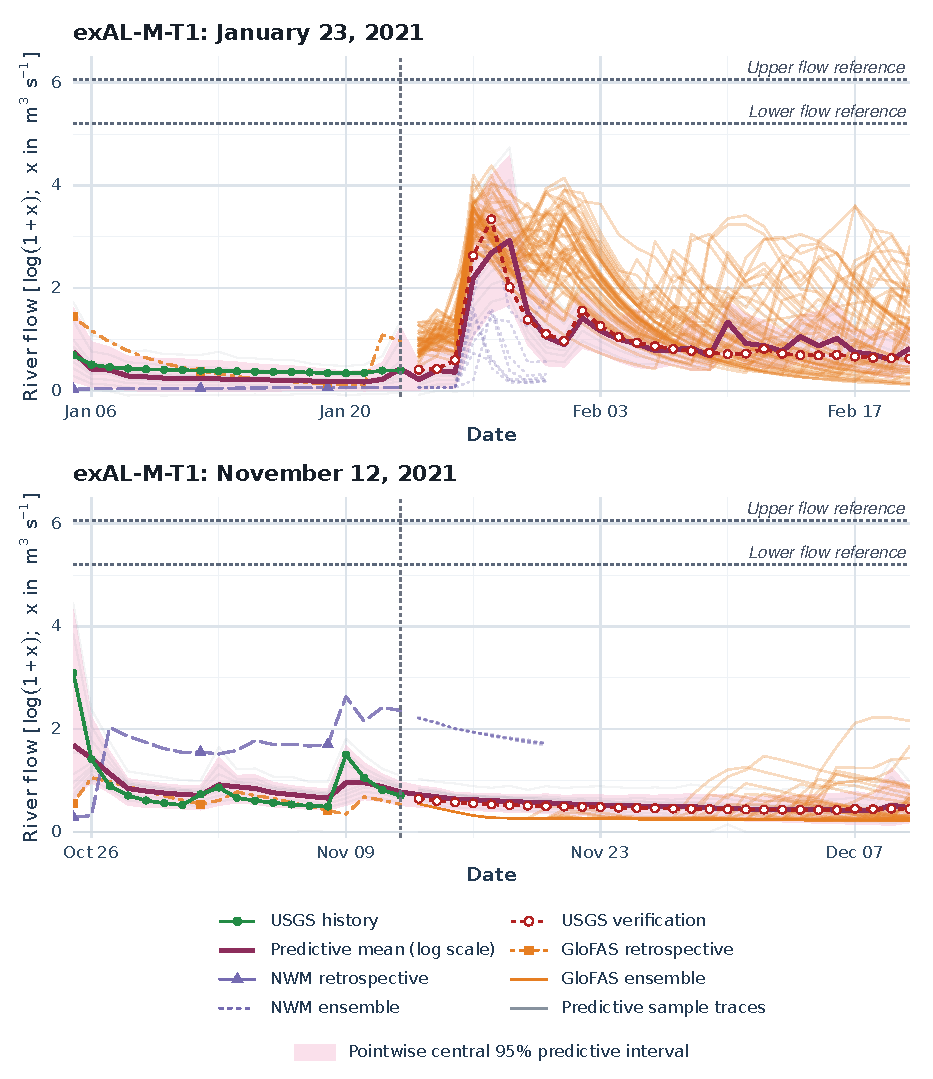
\includegraphics[width=450pt]{compact_forecasts_2021_early.pdf}
\caption{Reference exAL-M-T1 predictions at January 23 and November 12, 2021, on the $\log(1+x)$ scale, $x$ in m$^3$/s. Colors, symbols, sample traces and pointwise central 95\% intervals match Figure~\ref{fig:synth1}, with one shared legend and the common vertical range -0.1 to 6.5. The vertical line marks the origin $T$ and the first target is $T+1$.}
\label{fig:forecast_origins_2021_early}
\end{figure}
\begin{figure}[p]
\centering
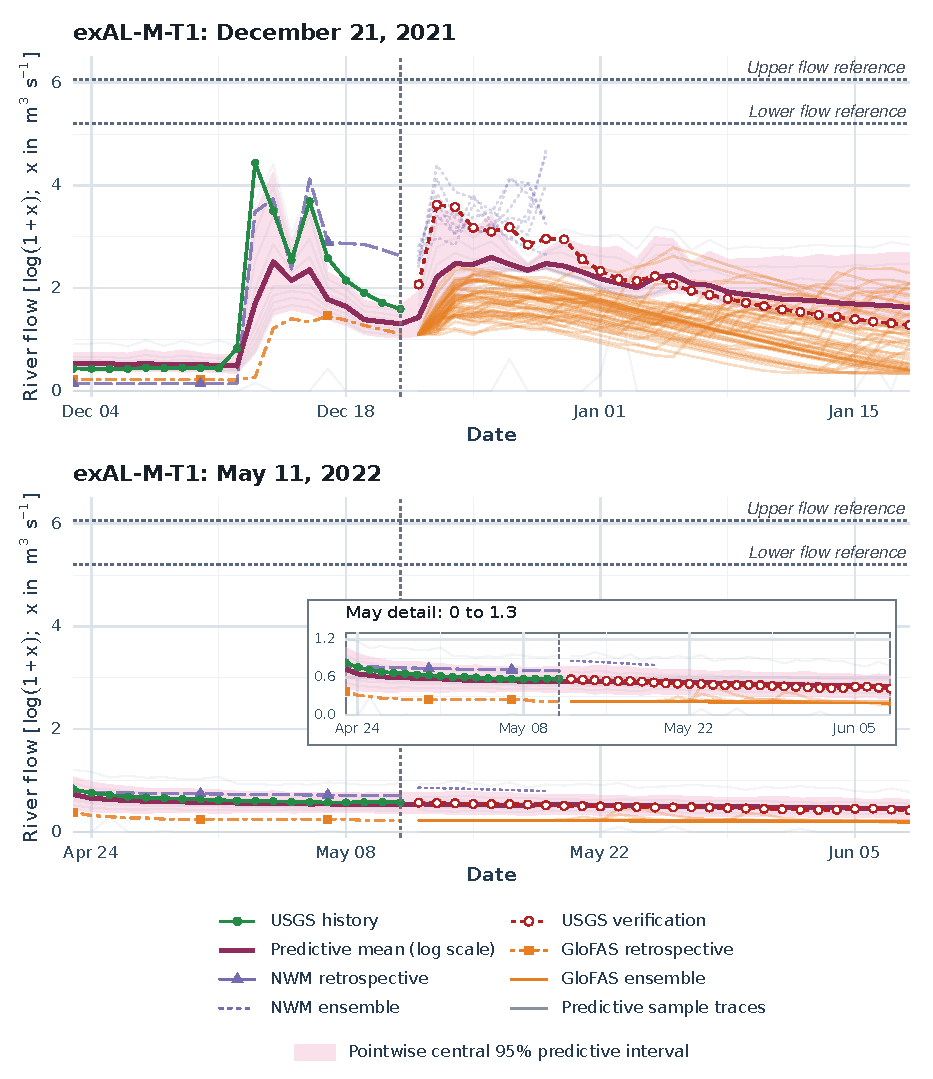
\includegraphics[width=450pt]{compact_forecasts_2021_2022.pdf}
\caption{Reference exAL-M-T1 predictions at December 21, 2021 and May 11, 2022. Graphical conventions and the common vertical scale match Figures~\ref{fig:synth1} and \ref{fig:forecast_origins_2021_early}. The labeled May inset displays the same predictions and source products over the range 0--1.3 to show low-flow variation.}
\label{fig:forecast_origins_2021_2022}
\end{figure}
\section{State-Space Construction and Computational Details}
\label{app:stateconstruction}

\subsection{Computing Time}
\label{app:computationtime}

AL and exAL fits use mean-field variational Bayes (VB); Gaussian variants use Gaussian filtering and smoothing. For the daily record in this application, seven independent quantile fits run in parallel; their representative combined fitting and forecasting time is approximately two hours on a Linux server with 64 cores and 503 GiB of memory, after preparation of the observation and covariate series. The two stages were not timed separately. Computing time depends on the hardware, implementation, series length and state dimension.

\subsection{Seasonal Rotations}
\label{app:seasonalconstruction}

For daily time steps, the seasonal specification uses a base period \(P=363.5854\) days and frequency multipliers \(h_1=1\), \(h_2=2\), and \(h_3=1/6.8068493\). The daily angular frequencies are \(\omega_a=2\pi h_a/P\), with rotation matrix
\[
\mathbf R(\omega)=
\begin{bmatrix}\cos\omega&\sin\omega\\-\sin\omega&\cos\omega\end{bmatrix}.
\]
The corresponding periods are approximately 363.59, 181.79, and 2474.87 days; the last is about 6.78 calendar years, or 81.3 months. These are the periods of the fitted daily rotations. With \(\mathbf E_2=(1,0)'\), the observation loading and transition are
\[
\mathbf F_t=(1,\mathbf E_2',\mathbf E_2',\mathbf E_2')',\qquad
\mathbf G_t=\operatorname{BlockDiag}\{1,\mathbf R(\omega_1),\mathbf R(\omega_2),\mathbf R(\omega_3)\},
\]
so \(p=7\), \(\mathbf F_t\in\mathbb R^7\), and \(\mathbf G_t\in\mathbb R^{7\times7}\).

\subsection{Predictive Synthesis and Empirical Quantiles}
\label{app:numericalprediction}

The initial synthesized quantile curve in the predictive synthesis is evaluated at 1,001 internal probability-grid points. Its values are sorted for monotone rearrangement, and inverse cumulative distribution function (CDF) sampling produces 2,000 draws per time. Linear interpolation is used between the grid values and constant interpolation beyond the two endpoints. Beyond the lowest and highest fitted probabilities, 0.05 and 0.95, the construction uses the corresponding outer fitted predictive distributions. Consequently, the limits of a central 95\% predictive interval are not separately fitted 0.025 and 0.975 model quantiles.

For ordered predictive values \(x_{(1)}\leq\cdots\leq x_{(n)}\), an interpolated empirical quantile is \((1-g)x_{(j)}+g x_{(j+1)}\), where \(j=\lfloor h\rfloor\), \(g=h-j\), and the minimum and maximum are used beyond the corresponding endpoints. The predictive quantiles from individual fits used for isotonic projection and synthesis take \(h=1+(n-1)u\), conventionally called type 7. The additional stochastic-model quantiles used for the calibration assessment and the displayed model-interval limits take \(h=(n+1/3)u+1/3\), conventionally called type 8 \citep{hyndman1996sample}. The four principal quantile competitors use the same predictive quantiles in the check-loss and reliability comparisons. Raw ensembles and deterministic quantile grids use the empirical generalized inverse, \(x_{(\lceil nu\rceil)}\) for \(0<u\leq1\), with the minimum at \(u=0\). These conventions specify finite-sample calculations without changing the fitted models.

% WIS rank-pairing identity and normalization.
For the ordered predictive values used in Subsection~\ref{subsec:distributionchecks}, write \(C_S=(2/S)\sum_{s=1}^S\rho_{s/(S+1)}(y-x_{(s)})\). Let \(K=\lfloor S/2\rfloor\), \(\alpha_k=2k/(S+1)\), \(l_k=x_{(k)}\) and \(u_k=x_{(S+1-k)}\), for \(k=1,\ldots,K\). With \(\alpha\) denoting excluded tail probability, the central interval score is
\[
\mathrm{IS}_{\alpha}(l,u;y)=(u-l)+\frac2\alpha(l-y)\mathbf1(y<l)
+\frac2\alpha(y-u)\mathbf1(y>u).
\]
Symmetric check losses satisfy
\[
\rho_{\alpha_k/2}(y-l_k)+\rho_{1-\alpha_k/2}(y-u_k)
=\frac{\alpha_k}{2}\mathrm{IS}_{\alpha_k}(l_k,u_k;y).
\]
Consequently,
\[
C_S=\begin{cases}
\displaystyle\frac1K\sum_{k=1}^K\frac{\alpha_k}{2}\mathrm{IS}_{\alpha_k}(l_k,u_k;y),&S=2K,\\[6pt]
\displaystyle\frac{\tfrac12|y-x_{(K+1)}|+\sum_{k=1}^K\tfrac{\alpha_k}{2}\mathrm{IS}_{\alpha_k}(l_k,u_k;y)}{K+\tfrac12},&S=2K+1.
\end{cases}
\]
The odd case is the conventional median-inclusive weighted interval score \citep{bracher2021evaluating}; the even case has no separate median term. These identities concern the assigned rank levels of the full predictive representation, not just the seven fitted probabilities. They do not identify the quantile-grid approximation with exact empirical-distribution CRPS.
% End WIS rank-pairing identity and normalization.

For the equally weighted empirical distribution $G_m=m^{-1}\sum_{i=1}^m\delta_{x_i}$, define
\[
A=\frac1m\sum_{i=1}^m|x_i-y|,\qquad
D=\sum_{i<j}|x_i-x_j|.
\]
The exact empirical-distribution score and separate independent-draw adjustment are
\[
\mathrm{CRPS}(G_m,y)=A-\frac{D}{m^2},\qquad
\mathrm{CRPS}_{\rm adj}=A-\frac{D}{m(m-1)}.
\]
The quantile-grid score in Subsection~\ref{subsec:distributionchecks} equals the exact score plus $D/[m^2(m+1)]$, explaining their difference on the same predictive values \citep{zamo2018crps}. The adjusted score estimates the parent-distribution CRPS under independent, identically distributed draws \citep{ferro2014fair}; that assumption is additional for physical ensembles. The adjustment is inapplicable to deterministic quantile grids and point masses. Exact skill uses the matching exact climatology denominator; no adjusted skill is reported.

\subsection{EMOS Optimization}
\label{app:emoscomputation}

For each lead, the EMOS fit minimizes the analytic truncated-normal CRPS over the eligible training cases described in Subsection~\ref{subsec:externalreferences}. We use four deterministic initial values and bounded limited-memory Broyden--Fletcher--Goldfarb--Shanno optimization (L-BFGS-B), retaining the converged solution with the lowest objective. The constraints are \(b,d\geq0\) and \(c>0\) in the location and variance parameterization. Training cases, numerical scaling and bounds, fitted parameter values, convergence criteria and boundary assessments are included in the reproducibility materials.

\subsection{Stacked States and Selectors}
\label{app:stackedstates}

For target probability $p_0$, $\operatorname{exAL}_{p_0}(\mu,\sigma,\gamma)$ denotes the extended asymmetric Laplace working likelihood with quantile location $\mu$, scale $\sigma>0$ and skewness $\gamma$ in the domain defined below. Each quantile model uses a shared $p$-dimensional trend/seasonal state $\boldsymbol\theta_t$, source discrepancies $\boldsymbol\delta_t^j$ and an $(m+1)$-dimensional transfer block. Let $\mathcal J=\{1,\ldots,J\}$ index external sources; source $j$ has members $i\in\mathcal I_j=\{1,\ldots,I_j\}$ and leads $k\in\mathcal K_j=\{1,\ldots,K_{(j)}\}$, with $K_{\max}=\max_jK_{(j)}$. The loading $\mathbf F_t$ and transition $\mathbf G_t$ have dimensions $p$ and $p\times p$. Stack
\[
\boldsymbol{\omega}_t' = [\zeta_t,\ \boldsymbol{\psi}_t'], \qquad
\boldsymbol{\eta}_t' = [\boldsymbol{\theta}_t',\ (\boldsymbol{\delta}_t^1)',\ \ldots,\ (\boldsymbol{\delta}_t^J)',\ \boldsymbol{\omega}_t'],
\]
where \(\boldsymbol{\omega}_t \in \mathbb{R}^{m+1}\) and \(\boldsymbol{\eta}_t \in \mathbb{R}^{q}\), with \(q = (J+1)\cdot p + m + 1\). The transfer update can be written as
\[
\mathbf{G}^{\text{trans}}_t =
\begin{bmatrix}
\lambda & \mathbf{x}_t' \\
\mathbf{0}_m & \mathbf{I}_m
\end{bmatrix}.
\]
Let $\mathcal J=\{1,\ldots,J\}$ and \(\mathcal{J}_0=\{0\}\cup\mathcal{J}\), where \(s=0\) denotes the USGS observation channel and \(s\in\mathcal{J}\) denotes an external product family. Let \(y_t^0 \equiv y_t^o\) denote the observation channel and \(y_t^s \equiv z_t^s\), \(s\in\mathcal{J}\), denote the retrospective-product channels. The corresponding compact form is:
\begin{alignat}{3}
\text{Pre-cutoff observations:}\quad&
y_t^s \mid \boldsymbol{\eta}_t, \sigma^s, \gamma^s
&\sim{}& \text{exAL}_{p_0}\!\left(\mathbf{h}_{t,s}' \boldsymbol{\eta}_t, \sigma^s, \gamma^s\right),
&\qquad& 1 \le t \le T,\ s \in \mathcal{J}_0, \label{eq:compact_est_obs}
\\
\text{Pre-cutoff state evolution:}\quad&
\boldsymbol{\eta}_t \mid \boldsymbol{\eta}_{t-1}
&\sim{}& \mathcal{N}\!\left(\boldsymbol{D}_t \boldsymbol{\eta}_{t-1}, \boldsymbol{\Lambda}_t\right),
&\qquad& 1 \le t \le T, \label{eq:compact_est_state}
\\
\text{Forecast observations:}\quad&
y_T^{j,i}(k) \mid \boldsymbol{\eta}_{T+k}, \sigma^j, \gamma^j
&\sim{}& \text{exAL}_{p_0}\!\left(\mathbf{e}_{T+k,j}' \boldsymbol{\eta}_{T+k}, \sigma^j, \gamma^j\right),
&\qquad& j \in \mathcal{J},\ i \in \mathcal{I}_j,\ k \in \mathcal{K}_j, \label{eq:compact_fc_obs}
\\
\text{Forecast state evolution:}\quad&
\boldsymbol{\eta}_{T+k} \mid \boldsymbol{\eta}_{T+k-1}
&\sim{}& \mathcal{N}\!\left(\boldsymbol{M}_{T+k} \boldsymbol{\eta}_{T+k-1}, \mathbf{W}_{T+k}\right),
&\qquad& 1 \le k \le K_{\max}. \label{eq:compact_fc_state}
\end{alignat}

Here
\[
\big(\mathbf{F}_t^{\text{trans}}\big)' = [1,\ \mathbf{0}_m'], \qquad
\mathbf{h}_{t,0}' =
\big[\mathbf{F}_t',\ \mathbf{0}_{pJ}',\ \big(\mathbf{F}_t^{\text{trans}}\big)'\big],
\qquad
\mathbf{h}_{t,j}' =
\big[\mathbf{F}_t',\ \mathbf{0}_{p(j-1)}',\ \mathbf{F}_t',\ \mathbf{0}_{p(J-j)}',\ \big(\mathbf{F}_t^{\text{trans}}\big)'\big],
\quad j \in \mathcal{J},
\]
with \(\mathbf{F}_t^{\text{trans}} \in \mathbb{R}^{m+1}\), \(\mathbf{h}_{t,0}, \mathbf{h}_{t,j} \in \mathbb{R}^{q}\), and
\[
\boldsymbol{D}_t = \text{BlockDiag}\!\left(\mathbf{G}_t,\ \underbrace{\mathbf{G}_t,\ldots,\mathbf{G}_t}_{J\ \text{discrepancy blocks}},\ \mathbf{G}^{\text{trans}}_t\right), \qquad
\boldsymbol{\Lambda}_t = \text{BlockDiag}\!\left(\mathbf{W}^{\theta}_t,\ \underbrace{\mathbf{W}^{\delta^1}_t,\ldots,\mathbf{W}^{\delta^J}_t}_{J\ \text{source-specific discrepancy blocks}},\ \text{BlockDiag}\!\left(w_t^{\zeta}, \mathbf{W}^{\psi}_t\right)\right),
\]
where \(\boldsymbol{D}_t, \boldsymbol{\Lambda}_t \in \mathbb{R}^{q\times q}\) and \(\sigma^s \in \mathbb{R}_+\), \(\gamma^s \in \mathbb{R}\) denote the channel-specific scale and skewness parameters for \(s \in \mathcal{J}_0\). Thus, \(\mathbf{h}_{t,0}' \boldsymbol{\eta}_t = \mathbf{F}_t' \boldsymbol{\theta}_t + \zeta_t\) and \(\mathbf{h}_{t,j}' \boldsymbol{\eta}_t = \mathbf{F}_t'(\boldsymbol{\theta}_t + \boldsymbol{\delta}_t^j) + \zeta_t\). For the forecast window, \(\mathbf{e}_{T+k,j}\) is the analogue of \(\mathbf{h}_{t,j}\): it extracts the latent trend-and-seasonal block, the discrepancy block for source \(j\), and the transfer block. For \(t>T\), \(\boldsymbol M_t\) denotes the forecast transition constructed from the same blocks as \(\boldsymbol D_t\): the trend-and-seasonal block, the discrepancy blocks of active sources, and \(\mathbf G_t^{\mathrm{trans}}\) evaluated with \(\mathbf x_t\). At a change in source availability, the preceding state is first restricted to the retained coordinates. State vectors, selectors and covariance matrices are restricted consistently. The full dimension is \(q\); the active dimension is denoted by \(p_t\) in Subsection~\ref{app:forecastcovariance}.

The augmentation in Subsection~\ref{app:augmentation} makes the observation equations conditionally Gaussian, while the state evolution remains Gaussian. The model can therefore be handled with standard state-space methods, including filtering, smoothing, and sampling recursions.

\subsection{Extended Asymmetric Laplace Augmentation}
\label{app:augmentation}

For fixed \(p_0\), the skewness bounds are the negative root \(L_\gamma(p_0)\) of \(g(\gamma)=1-p_0\) and positive root \(U_\gamma(p_0)\) of \(g(\gamma)=p_0\), where
\[
g(\gamma)=2\Phi(-|\gamma|)\exp(\gamma^2/2).
\]
Here \(\Phi\) is the standard normal cumulative distribution function. These bounds ensure \(0<p(\gamma;p_0)<1\) for
\[
p(\gamma;p_0)=I(\gamma<0)+\{p_0-I(\gamma<0)\}/g(\gamma).
\]
The functions used in the algorithms are
\[
A(\gamma;p_0)=\frac{1-2p(\gamma;p_0)}{p(\gamma;p_0)\{1-p(\gamma;p_0)\}},\qquad
B(\gamma;p_0)=\frac{2}{p(\gamma;p_0)\{1-p(\gamma;p_0)\}},\qquad
C(\gamma;p_0)=\{I(\gamma>0)-p(\gamma;p_0)\}^{-1}.
\]
Using independent \(e\sim\mathcal N(0,1)\), \(u\sim\operatorname{Exp}(1)\), and \(s\sim\mathcal N^+(0,1)\), where the last distribution is truncated to the positive half-line, \citet{yan2025new} give the representation
\[
Y=\mu+C(\gamma;p_0)\sigma|\gamma|s+A(\gamma;p_0)\sigma u+
\sqrt{B(\gamma;p_0)\sigma^2u}\,e.
\]
The algorithms use $v=\sigma u$, so the conditional Gaussian variance is $B(\gamma;p_0)\sigma v$. We use the generalized inverse-Gaussian convention
\[
\mathcal{GIG}(p,a,b)\propto x^{p-1}\exp\{-(ax+b/x)/2\},\qquad x>0.
\]
The positive-truncated normal distribution is denoted by $\mathcal N^+$. The second argument of \(\mathcal N^+\) in the algorithms is the underlying Gaussian variance. This separates the augmentation variables from the retrospective products \(z_t^j\), and the Gaussian noise \(e\) from the covariance-prior weight \(\epsilon\).

\subsection{Forecast-Window Covariance Prior}
\label{app:forecastcovariance}

During the forecast window ($t \in \{T+1, \ldots, T+K_{\max}\}$), we set the Inverse Wishart prior parameters as $\mathbf{S}_t = (\nu_t - p_t - 1)\, c\, \mathbf{W}_T$ and $\nu_t = (p_t + 1 + \epsilon)$, with $\epsilon, c > 0$, where \(p_t\) denotes the dimension of the active forecast-window state at time \(t\), \(\mathbf{S}_t \in \mathbb{R}^{p_t\times p_t}\), and \(\mathbf{W}_T \in \mathbb{R}^{p_t\times p_t}\) after restricting the full pre-cutoff covariance to the active forecast-window block. Under this specification, the posterior mean is
\(
\mathbb{E}[\mathbf{W}_t \mid \mathcal{D}_t] = \frac{\epsilon}{1 + \epsilon}(c\, \mathbf{W}_T) + \frac{1}{1 + \epsilon} \mathbb{E}\left[ (\boldsymbol{\eta}_t - \boldsymbol{M}_t \boldsymbol{\eta}_{t-1}) (\boldsymbol{\eta}_t - \boldsymbol{M}_t \boldsymbol{\eta}_{t-1})' \mid \mathcal{D}_t \right],
\)
where $\mathcal{D}_t$ denotes all data available up to and including time $t$.

The inverse-Wishart convention has mean $\mathbf S_t/(\nu_t-p_t-1)$. The weights stabilize covariance estimation from the available forecast-product updates. To evaluate the innovation expectation, write $\bar{\mathbf e}_t=\mathbf m_t^s-\mathbf M_t\mathbf m_{t-1}^s$ and $\mathbf C_{t,t-1}^s=\operatorname{Cov}(\boldsymbol\eta_t,\boldsymbol\eta_{t-1})$. Then
\[
\mathbb E(\mathbf e_t\mathbf e_t')=
\bar{\mathbf e}_t\bar{\mathbf e}_t'+\mathbf C_t^s+
\mathbf M_t\mathbf C_{t-1}^s\mathbf M_t'
-\mathbf C_{t,t-1}^s\mathbf M_t'-\mathbf M_t(\mathbf C_{t,t-1}^s)'.
\]
With the smoothing gains in Algorithm~\ref{alg:Alg4}, $\mathbf C_{t,t-1}^s=\mathbf C_t^s\mathbf B_{t-1}'$. All quantities are restricted consistently when the active state dimension changes.

\subsection{Laplace--Delta Approximation}
\label{app:vblad}

The variational Bayes Laplace--Delta (VB-LD) approximation updates scale and skewness jointly. Let \(\mathcal D\) denote the observation values entering the specified likelihood. Let \(\boldsymbol\alpha\) collect unconstrained scale and skewness parameters for one channel, and let \(\boldsymbol\beta\) collect the remaining unknown quantities, whose current variational density is \(r(\boldsymbol\beta)\). The non-conjugate coordinate update has log kernel
\(\ell(\boldsymbol\alpha)=\mathbb E_{r(\boldsymbol\beta)}[\log p(\mathcal D,\boldsymbol\alpha,\boldsymbol\beta)]\).
A Laplace approximation sets
\[
r(\boldsymbol\alpha)\approx\mathcal N(\widehat{\boldsymbol\alpha},\boldsymbol\Sigma),\qquad
\widehat{\boldsymbol\alpha}=\arg\max\ell(\boldsymbol\alpha),\qquad
\boldsymbol\Sigma=-\{\nabla^2\ell(\widehat{\boldsymbol\alpha})\}^{-1}.
\]
For a nonlinear function \(g\), the second-order Delta approximation supplies
\[
\mathbb E_r[g(\boldsymbol\alpha)]\approx g(\widehat{\boldsymbol\alpha})+
\tfrac12\operatorname{Tr}\{\nabla^2g(\widehat{\boldsymbol\alpha})\boldsymbol\Sigma\}.
\]
These moments enter the conditionally conjugate state and augmentation updates in Algorithms~\ref{alg:Alg3} and \ref{alg:Alg4}. Conditional on the evolution covariances, the factorization is
\[
r(\boldsymbol\eta_{0:T+K_{\max}})\prod_{a\in\mathcal A}r(v_a)r(s_a)
\prod_{j\in\mathcal J_0}r(\sigma^j,\gamma^j),
\]
Here $\mathcal A$ indexes available observations, including each active forecast member. Dependence between scale and skewness is retained within each channel's Laplace factor.

\section{Variational Bayes Updates}
\label{app:vbupdates}

Algorithms~\ref{alg:Alg3} and \ref{alg:Alg4} display historical-window coordinate updates and Gaussian state recursions. Initialize state moments from $\mathcal N(\mathbf m_0,\mathbf C_0)$ and initialize augmentation and channel-parameter moments before the first outer iteration. Angle brackets denote expectations under the current variational factors; $\mathcal L$ denotes the evidence lower bound (ELBO). The same observation-level updates apply to each available forecast member after replacing $(t,j)$ by $(T+k,j,i)$ and using the corresponding selector and active-state transition. In the forecast window, an observation vector stacks all active pairs \((j,i)\), where \(j\) identifies a source and \(i\) a member. Selector columns repeat within a source, while each member has its own augmentation variables. A source-specific parameter objective includes every retrospective value and available issued member: with complete historical support this gives \(T+I_jK_{(j)}\) contributions for external source \(j\), and \(T\) for the gauge channel. Forecast state evolution uses the covariance specification in Subsection~\ref{app:forecastcovariance}.

\begin{algorithm}
\caption{Historical-window variational Bayes (VB) coordinate updates}
\label{alg:Alg3}
\begin{algorithmic}

\State \textbf{Notation:}
\State  $\left\langle g(\xi) \right\rangle = \mathbb{E}_\xi\left[ g(\xi) \right]$
\State  \(
A^j = A(\gamma^j;p_0), \quad B^j = B(\gamma^j;p_0), \quad C^j = C(\gamma^j;p_0), \text{ as defined in Subsection~\ref{app:augmentation}}
\)
\State  Let \(\mathcal{J}_0=\{0\}\cup\mathcal{J}\). During the pre-cutoff observation window, let \(y_t^0 \equiv y_t^o\) and \(y_t^j \equiv z_t^j\) for \(j\in\mathcal{J}\), with selector \(\mathbf{h}_{t,j}\).
\State \textbf{Step 0: Set initial values}
\State Choose \(k_{\max}\), minimum update counts, and convergence tolerances; set \(k=0\)

\While{\(k < k_{\max}\) and convergence criteria are not met}
    \State \(k \leftarrow k+1\)
    \State \textbf{Step 1: Update $r(\boldsymbol{\eta}_t)=\mathcal{N}(\mathbf m^{(k)}_t,\mathbf C^{(k)}_t)$}
    \State Use Algorithm~\ref{alg:Alg4}

    \For{$j \in \mathcal{J}_0$}
        \State \textbf{Step 2: Update $r(v^j_t)=\mathcal{GIG}(a_t^{j,(k)},b_t^{j,(k)},c_t^{j,(k)})$}
        \For{$t = 1$ to $T$}
            \State $a_t^{j,(k)} = \frac{1}{2}$
            \State $b_t^{j,(k)} = \left\langle \frac{(A^j)^2}{\sigma^j B^j} \right\rangle^{(k-1)} + 2 \left\langle \frac{1}{\sigma^j} \right\rangle^{(k-1)}$
            \State $c_t^{j,(k)} = \left\langle \frac{1}{\sigma^j B^j} \right\rangle^{(k-1)} \Big[ (y_t^j)^2 - 2y_t^j \left\langle  \mathbf{h}_{t,j}' \boldsymbol{\eta}_t \right\rangle^{(k)} + \left\langle (  \mathbf{h}_{t,j}' \boldsymbol{\eta}_t )^2 \right\rangle^{(k)} \Big]$
            \State $\quad \quad -2 \left\langle s^j_t \right\rangle^{(k-1)} \left\langle \frac{C^j|\gamma^j|}{B^j} \right\rangle^{(k-1)} \Big[ y_t^j - \left\langle  \mathbf{h}_{t,j}' \boldsymbol{\eta}_t \right\rangle^{(k)} \Big]$
            \State $\quad \quad + \left\langle (s^j_t)^2 \right\rangle^{(k-1)} \left\langle \frac{(C^j)^2\sigma^j|\gamma^j|^2}{B^j} \right\rangle^{(k-1)}$
        \EndFor

        \State \textbf{Step 3: Update $r(s^j_t)=\mathcal{N}^+(a_{s,t}^{j,(k)},\ell_t^{j,(k)})$}
        \For{$t = 1$ to $T$}
            \State $\ell_t^{j,(k)} = \Big[ 1+\left\langle \frac{(C^j)^2 \sigma^j |(\gamma^j)|^2}{B^j} \right\rangle^{(k-1)} \left\langle \frac{1}{v^j_t} \right\rangle^{(k)} \Big]^{-1}$
            \State $a_{s,t}^{j,(k)} = \ell_t^{j,(k)}  \Big[ \left\langle \frac{C^j |\gamma^j|}{B^j} \right\rangle^{(k-1)} \left\langle \frac{1}{v^j_t} \right\rangle^{(k)} \Big( y_t^j - \left\langle  \mathbf{h}_{t,j}' \boldsymbol{\eta}_t \right\rangle^{(k)} \Big) - \left\langle \frac{C^j |\gamma^j| A^j}{B^j} \right\rangle^{(k-1)} \Big]$
        \EndFor

        \State \textbf{Step 4: Update $r(\gamma^j, \sigma^j )$}
        \State Approximate via VB-LD, as described in Subsection~\ref{app:vblad}
    \EndFor
    \State \textbf{Step 5: Check convergence}
    \State Compute \(\mathcal{L}^{(k)}\), \(\Delta_{\mathcal{L}}^{(k)}=|\mathcal{L}^{(k)}-\mathcal{L}^{(k-1)}|\), and the relative ELBO change
    \State Declare convergence after required update iterations when ELBO,
    \Statex \hspace{\algorithmicindent} state, scale, and skewness changes are below their tolerances
\EndWhile

\end{algorithmic}
\end{algorithm}

\begin{algorithm}
\caption{VB-Filtering and VB-Smoothing}
\label{alg:Alg4}
\begin{algorithmic}

\State \textbf{Notation:}
\State $\left\langle g(\xi) \right\rangle = \mathbb{E}_\xi\left[ g(\xi) \right]$
\State  During the pre-cutoff observation window, \(\mathbf{H}_t = [\mathbf{h}_{t,0}, \mathbf{h}_{t,1}, \ldots, \mathbf{h}_{t,J}]\), \(\mathbf{Y}_t = [y_t^o, z_t^1, \ldots, z_t^J]'\), and \(\mathbf{D}_t, \boldsymbol{\Lambda}_t\) are as defined in Subsection~\ref{app:stackedstates}.
\State  Equivalently, let \(y_t^0 \equiv y_t^o\) and \(y_t^j \equiv z_t^j\) for \(j\in\mathcal{J}\).
\State For each active channel, define the expected precision and weighted offset:
\State $\pi_t^j=\left\langle\frac{1}{B^j\sigma^jv_t^j}\right\rangle$
\State $b_t^j=(\pi_t^j)^{-1}\left\langle\frac{C^j\sigma^j|\gamma^j|s_t^j+A^jv_t^j}{B^j\sigma^jv_t^j}\right\rangle$
\State $\mathbf b_t=[b_t^j]_{j\in\mathcal J_0}$, \quad $\mathbf O_t=\operatorname{Diag}\big([(\pi_t^j)^{-1}]_{j\in\mathcal J_0}\big)$
\State At outer iteration \(k\), augmentation and parameter moments are from iteration \(k-1\); the smoothed moments below define \(\mathbf m_t^{(k)},\mathbf C_t^{(k)}\).
\State \(A^j,B^j,C^j\) are defined in Subsection~\ref{app:augmentation}.
\State \textbf{Step 1: Forward Filtering}
\For{$t = 1$ to $T$}
    \State Compute Prior moments:
    \State $\mathbf{a}_t = \mathbf{D}_t \mathbf{m}_{t-1}$
    \State $\mathbf{R}_t = \mathbf{D}_t \mathbf{C}_{t-1} \mathbf{D}_t' +  \boldsymbol{\Lambda}_t$

    \State One-step-ahead forecast:
    \State $\mathbf{f}_t = \mathbf{H}_t'\mathbf{a}_t + \mathbf{b}_t$
    \State $\mathbf{Q}_t = \mathbf{H}_t'\mathbf{R}_t\mathbf{H}_t + \mathbf{O}_t$

    \State Compute Posterior moments:
    \State $\mathbf{m}_t = \mathbf{a}_t + \mathbf{R}_t \mathbf{H}_t \mathbf{Q}_t^{-1}(\mathbf{Y}_t - \mathbf{f}_t)$
    \State $\mathbf{C}_t = \mathbf{R}_t - \mathbf{R}_t \mathbf{H}_t \mathbf{Q}_t^{-1} \mathbf{H}_t' \mathbf{R}_t$
\EndFor

\State \textbf{Step 2: Backward Smoothing}
\For{$t = T$ down to $1$}
    \If{$t = T$}
        \State Set $r^{(k)}(\boldsymbol{\eta}_T) := \mathcal{N}(\mathbf{m}_T^s, \mathbf{C}_T^s)$
        \State $\mathbf{m}_T^s = \mathbf{m}_T$
        \State $\mathbf{C}_T^s = \mathbf{C}_T$
    \Else
        \State Compute Smoothing moments:
        \State $r^{(k)}(\boldsymbol{\eta}_t) := \mathcal{N}(\mathbf{m}_t^s, \mathbf{C}_t^s)$
        \State $\mathbf{B}_t = \mathbf{C}_t \mathbf{D}_{t+1}' \mathbf{R}_{t+1}^{-1}$
        \State $\mathbf{m}_t^s = \mathbf{m}_t + \mathbf{B}_t (\mathbf{m}_{t+1}^s - \mathbf{a}_{t+1})$
        \State $\mathbf{C}_t^s = \mathbf{C}_t + \mathbf{B}_t (\mathbf{C}_{t+1}^s - \mathbf{R}_{t+1}) \mathbf{B}_t'$
    \EndIf
\EndFor


\end{algorithmic}
\end{algorithm}

\FloatBarrier
\end{appendix}

\bibliography{wileyNJD-APA}
\end{document}
